\documentclass[letterpaper]{article}
\usepackage[us]{datetime}
\usepackage{CJKutf8}
\usepackage[T1,T2A]{fontenc}
\usepackage[utf8]{inputenc}
\usepackage{varwidth}
\usepackage{lastpage}
\usepackage{fancyhdr}
\usepackage{appendix}
\settimeformat{ampmtime}
\pagestyle{fancy}
\newcommand{\myfooters}{
\rfoot{\small electronic mail\\ \url{mailto:justina@colmena.biz?subject=P_vs_NP}}
\cfoot{\small \textbf{[\begin{NoHyper}Page\ \thepage\ of\ \pageref{LastPage}\end{NoHyper}]}}
\lfoot{\small justina colmena\\\today\ @\currenttime}
\renewcommand{\footrulewidth}{\headrulewidth}
}
\myfooters

\fancypagestyle{plain}{
	\fancyhf{}
	\lhead{\textit{TITLE PAGE}}
	\rhead{\textit{Nothing to see here.  Please move along.}}
	\myfooters
}


%\usepackage{lmodern}
\usepackage[numbers]{natbib}
\usepackage[finnish,swedish,french,german,spanish,italian,russian,latin,english]{babel}
\bibliographystyle{plainnat}
\usepackage[hyphens,lowtilde]{url}
\usepackage{wrapfig}
\usepackage[justification=centering]{caption}
\usepackage{hyperref}
\hypersetup{
	colorlinks=true, %set true if you want colored links
	linktoc=all,     %set to all if you want both sections and subsections linked
	linkcolor=blue,  %choose some color if you want links to stand out
}
%\usepackage[hyphenbreaks]{breakurl}

\usepackage{color}   %May be necessary if you want to color links
\usepackage{amsmath}
\usepackage{amsfonts}
\usepackage{amssymb}
\usepackage{amsthm}
\usepackage{thmtools}


\usepackage{marvosym,wasysym,textcomp,dictsym}
\usepackage{mathrsfs}
\usepackage{algpseudocode}
\usepackage{algorithm}
\usepackage[]{backnaur}
\usepackage{newfloat}
%\usepackage{syntax}

%\grammarindent=80pt
\usepackage{scalerel}
\usepackage{graphicx}
\graphicspath{{images/}}
\usepackage{svg}
\renewcommand{\includesvg}[1]{%
\immediate\write18
 {inkscape --batch-process -D --export-latex #1.svg --export-filename=#1.pdf}%
	\input{#1.pdf_tex}%
}

\usepackage{float}

\newsavebox\Volleyball
\savebox\Volleyball{\includesvg{images/b14f1090776e99712331d0c24973afc6}}

\newcommand{\Axiom}{{\large\Bearing}}
\declaretheorem[numberwithin=section,qed={\Axiom}]{axiom}
\newcommand{\AxiomSchema}{{\large\LooseBearing}}
\declaretheorem[sibling=axiom,name=Axiom Schema,qed={\AxiomSchema}]{axiomschema}
\newcommand{\Theorem}{\raisebox{0.5ex}{\large\Beam}}
\declaretheorem[numberwithin=section,qed={\Theorem}]{theorem}
\newcommand{\Lemma}{{\large\FlatSteel}}
\declaretheorem[sibling=theorem,qed={\Lemma}]{lemma}
\newcommand{\Corollary}{\CircPipe}
\declaretheorem[sibling=theorem,qed={\Corollary}]{corollary}
\newcommand{\Definition}{\raisebox{-0.25ex}{\large\dsliterary}}
\declaretheorem[sibling=theorem,style=definition,qed={\Definition}]{definition}
\newcommand{\Circumlocution}{{\large\dsmedical\dsjuridical}}
\declaretheorem[sibling=theorem,style=definition,qed={\Circumlocution}]{circumlocution}
\newcommand{\Construction}{{\large\dsmathematical}}
\declaretheorem[sibling=theorem,style=definition,qed={\Construction}]{construction}
\newcommand{\Remark}{\raisebox{-0.125ex}{\large\Coffeecup}}
\declaretheorem[numbered=no,style=remark,qed={\Remark}]{remark}
\newcommand{\Exercise}{\raisebox{-0.75ex}[0ex][0ex]{\scaleto{\usebox{\Volleyball}}{3ex}}}
\declaretheorem[style=remark,qed={\Exercise}]{exercise}

\renewcommand{\qedsymbol}{\textbf{\textsc{q.e.d.}}}


%opening
\title{\textbf{Liars' oracles}\\ Relativizing the $P$ vs.\ $NP$ question}
\author{Justina Colmena\footnote{\url{https://www.colmena.biz/~justina/pnp/}, B.S. Mathematics, B.S. Computer Science: University of Alaska Fairbanks, of ``HAARP'' fame \cite[etc.]{haarp,haarp.net,begich2002angels,burks2010haarp,want2016haarp,smith1998haarp,freeland2014chemtrails} ... \url{mailto:justina@colmena.biz?subject=P_vs._NP}}}

\begin{document}
\sloppy
\phantomsection\addcontentsline{toc}{section}{Title}\maketitle
\phantomsection\addcontentsline{toc}{section}{Abstract}
\begin{abstract} {\color{red}\textbf{WORK IN PROGRESS:}}
A somewhat whimsical investigation into the possibility of the formal independence of the $P$ vs.\ $NP$ question based on an oracle of Hartmanis and Hopcroft.
\end{abstract}
\begin{figure}
	
\includegraphics[width=1.0\textwidth]{images/guy_fawkes_mask.jpg}
	\caption[\texttt{(float)0x63/0x64}]{\texttt{(float)0x63/0x64} \cite{anon2012}}
\end{figure}

\phantomsection\addcontentsline{toc}{section}{Contents}\tableofcontents

\phantomsection\addcontentsline{toc}{section}{List of Figures}\listoffigures

\phantomsection\addcontentsline{toc}{section}{List of Algorithms}\listofalgorithms

\phantomsection\addcontentsline{toc}{section}{List of Tables}\listoftables

\section{Copyright}
This work is placed in the public domain by its author.\footnote{\url{https://github.com/justinacolmena/pnp/blob/master/LICENSE}} Questions of attribution are academic, and not intended to be enforced by copyright law. The style of this document is mostly intended for working copy.  This author raises no objection to adaptation of this document or its style for commercial or other publication.  Other authors who wish to take a particular portion of this document and expand upon it at greater length into their own work are encouraged to do so. For this reason, \LaTeX\textsuperscript{\textregistered} source code\footnote{\url{https://github.com/justinacolmena/pnp}} is distributed with this original work.

Those who wish to cite this (unfinished) paper are encouraged to quote or paraphrase the portions they are referring to in sufficient detail that their work does not depend on this remaining exactly as it is.  They are encouraged to make their mathematical arguments on mathematical merits rather than engaging in \foreignlanguage{latin}{\textit{ad hominem}} arguments of one author's claim against another, unless the latter really is the subject they wish to address.

To compile this entire paper it is necessary to have Inkscape and ImageMagick installed, and to use the \texttt{-shell-escape} switch with \texttt{pdflatex}. For some reason, it seems necessary to specify \texttt{-shell-escape} \textit{before} other switches on the command line.
\section{Introduction}
The purpose of this article is to expand on some comments originally made online by the author in a somewhat offhand manner \cite{myinfo2016,myinfo2016a,annorlunda2016}.  We attempt to show that the $P$ vs.\ $NP$ question remains undecided by any formal system $F$ capable of sufficient arithmetic and not containing a proof of its own inconsistency.

This is a work in progress.



\section{Turing machines}
Turing machines are named after Alan Turing (1912--1954), Figure~\ref{turing}, the British computer scientist and code-breaker who was chemically castrated as punishment for homosexuality in spite of his valiant efforts that were not only crucial to winning the war but of great scientific merit in peacetime, given the freedom that victory affords us to study his and others' related work.  An inquisition has yet to be made into the formal verdict of his death by suicide.
\begin{figure}
	\centering
	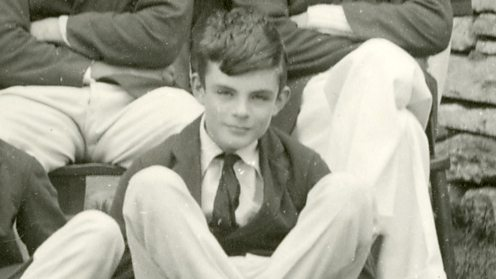
\includegraphics[width=1\textwidth]{images/alan-turing-school-photo.jpg}
	\caption[Alan Turing]{Alan Turing as a school-child \cite{hodges2017}.}
	\label{turing}
\end{figure}
\begin{definition}
A \textbf{deterministic accept/reject Turing machine} is a 'tuple
\begin{equation}
(\sigma,\Sigma,S,T,R,\delta),\label{dtuple}
\end{equation}
where $\sigma$ is a finite set of states, $\Sigma$ is a finite alphabet of at least two different symbols\footnote{$\Sigma=\{0,1\}$ is a minimal acceptable alphabet for a Turing machine.} that does not include the symbol $\triangleright$,\footnote{We do not teach, as do others, the so-called ``disjoint union'' \mbox{$\Sigma\sqcup\{\triangleright\}$}, which they attempt to define without regard to whether or not \mbox{$\triangleright\in\Sigma$}, since this is not a well-founded set by any of the axioms of Zermelo--Fraenkel set theory; we feel that it is necessary and sufficient to state explicitly that \mbox{$\triangleright\notin\Sigma$}. Those who have such a strong preference for the term ``disjoint union'' may simply state that the union \mbox{$\Sigma\cup\{\triangleright\}$} is disjoint because \mbox{$\Sigma\cap\{\triangleright\}=\emptyset$}.} $S\in\sigma$ is an initial or start state, $T\subset\sigma$ is a set of accepting final or halt states, $R\subset\sigma$ is a set of rejecting final or halt states, $T\cap R=\emptyset$, and $\delta$ is its \textbf{state transition table}, a function
\begin{equation}
\delta:\big((\sigma\backslash(T\cup R))\times(\Sigma\cup\{\triangleright\})\big)\longrightarrow\big((\Sigma\cup\{\triangleright\})\times\{\leftarrow,\rightarrow\}\times\sigma)\big)
\end{equation}
subject to the restrictions\footnote{The tick-mark after the delta $\delta`$ refers to an \textit{image} under the function $\delta$....}
\begin{align}
\delta`(\sigma\backslash(T\cup R)\times\{\triangleright\})&\subset \{\triangleright\}\times\{\rightarrow\}\times\sigma,\label{noback}\\
\delta`(\sigma\backslash(T\cup R)\times\Sigma)&\subset \Sigma\times\{\leftarrow,\rightarrow\}\times\sigma.\label{abuse1}
\end{align}
\end{definition}
\begin{remark}
Such a Turing machine is considered to have a tape, infinite in one direction only, readable and writable with the symbols of the alphabet $\Sigma$, and with the unique symbol \mbox{$\triangleright\notin\Sigma$} permanently engraved at the beginning of the tape.\footnote{The purpose of these restrictions is  to prevent the read/write head from (\ref{noback}) overwriting the symbol $\triangleright$ and backing off the beginning of the tape or (\ref{abuse1}) misusing the symbol $\triangleright$ in an inappropriate context: recall from (\ref{dtuple}) that \mbox{$\triangleright\notin\Sigma$}. If we were to omit the restriction (\ref{abuse1}), a Turing machines would be allowed to cut tape like a malfunctioning automatic cash register and leave receipts for various discarded intermediate computations all over the floor.}  The state transition table $\delta$ is interpreted to specify, for a given symbol read from the tape by the read/write head in a given state, a new symbol to be written to replace the symbol just read from the tape, a new direction to move the read/write head by one position on the tape, and a new state to enter upon completing this step of computation.
\end{remark}

\begin{definition}
A \textbf{non-deterministic Turing machine} is defined similarly, except that its state transition function is defined more generally
\begin{equation}
\Delta:\big((\sigma\backslash(T\cup R))\times(\Sigma\cup\{\triangleright\})\big)\longrightarrow\mathscr P\big((\Sigma\cup\{\triangleright\})\times\{\leftarrow,\rightarrow\}\times\sigma)\big)\backslash\{\emptyset\},
\end{equation}
subject to the restrictions
\begin{align}
\Delta`((\sigma\backslash(T\cup R))\times\{\triangleright\})&\subset\mathscr P\big(\{\triangleright\}\times\{\rightarrow\}\times\sigma\big)\backslash\{\emptyset\},\\
\Delta`((\sigma\backslash(T\cup R))\times\Sigma)&\subset\mathscr P \big(\Sigma\times\{\leftarrow,\rightarrow\}\times\sigma\big)\backslash\{\emptyset\},
\end{align}
which are straightforward generalizations of (\ref{noback}--\ref{abuse1}), where again, \mbox{$\triangleright\notin\Sigma$}, and $\mathscr P$ denotes the \textbf{power set} \mbox{$\mathscr P(X)=\{x|x\subset X\}$}.  See \Axiom \ref{powerset} and \AxiomSchema \ref{comprehensionschema}.
\end{definition}
\begin{definition}
An \textbf{alternating Turing machine} is a non-deterministic accept/reject Turing machine with some of its states (including the initial state) quantified as either universal or existential:  A path of computation leading into a universal state is considered to accept if and only if all possible paths continuing on from that state accept.  A path leading into an existential state is considered to accept if and only at least one path continuing on from that state accepts.
\end{definition}

\begin{definition}
	\textbf{Oracle or query machine?}
\end{definition}
\begin{definition}
	{\color{red}\textbf{Other variants...}}
\end{definition}

\section{Complexity classes}
\subsection{Formal definitions}
Information, references, and less formal definitions are available online at Scott Aaronson's ``Complexity Zoo'' \cite{aaronson-zoo}.
\subsubsection{Polynomial time}
\begin{definition}
A language $L\subset\Sigma^{*}$, where $\Sigma^{*}$ is the set of strings over some some finite alphabet $\Sigma$, is said to belong to the class $P$, i.e. $L\in P$ if there exist a deterministic Turing machine $M$ and a polynomial $p$, such that for all $s\in\Sigma^{*}$, the computation of $M$ begun from its initial state on the input $s$ terminates in a number of steps not more than $p(|s|)$,\footnote{By $|s|$ is denoted the \textit{length} of the string $s$.} in an accepting state whenever $s\in L$ and in a rejecting state whenever $s\notin L$.
\end{definition}
\begin{definition}
A language $L\subset\Sigma^{*}$, where $\Sigma^{*}$ is the set of strings over some some finite alphabet $\Sigma$, is said to belong to the class $NP$, i.e. $L\in NP$ if there exist a non-deterministic Turing machine $N$ and a polynomial $q$, such that for all $s\in\Sigma^{*}$, all possible paths of computation of $N$ beginning at its initial state on the input $s$ terminate in a number of steps not more than $q(|s|)$, at least one path in an accepting state whenever $s\in L$ and all paths in a rejecting state whenever $s\notin L$.
\end{definition}
\subsubsection{Exponential time}
\begin{definition}
The classes $EXP$ and $NEXP$ are defined similarly to $P$ and $NP$, except that the number of steps allowed for the computation is exponential in the polynomial, i.e., $2^{p(|s|)}$ and $2^{q(|s|)}$, respectively. It is known that $EXP=NEXP$ [\S \ref{bgsa}].
\end{definition}
\subsubsection{Recursion}
\begin{definition}
A language belongs to the class $PR$ of \textbf{primitive recursive} languages if it is recognizable by a deterministic Turing machine that halts on all inputs within a number of steps bounded by a \textit{primitive recursive function} \cite{robinson1949definability} of the length of the input.\footnote{The class of primitive recursive \textit{functions} is ``closed'' in a peculiar manner: any function, computable by a Turing machine in a number of steps bounded by a primitive recursive function of the length of the input, is itself primitive recursive.}
\end{definition}
\begin{definition}
A language belongs to the class $R$ of \textbf{general recursive} languages if it is recognizable by any deterministic Turing machine that halts on all inputs.  General recursive languages are simply called ``recursive'' when it is not necessary to emphasize the distinction from primitive recursive languages.
\end{definition}
\begin{definition}\label{def-re}
The class $RE$ of \textbf{recursively enumerable} languages is defined similarly to $R$, except that the Turing machine is not required to halt on inputs that do not belong to the language in question.
\end{definition}

\subsection{\textit{P} vs.\ \textit{NP}}

The $P$ vs.\ $NP$ question is at its root a philosophical question of whether or not an existentially quantified non-determinism, or even a bounded alternation between universal and existential states, ($P$ vs.\ $PH$ \cite{meurant2014algorithms},) properly extends the class of computational problems that may be solved in polynomial time.  Similar questions exist for other forms of non-determinism, such as those quantified not in an existential or universal sense but by classical probability measures, (e.g.,\ $ZPP=RP\operatorname\cap\textrm{co-}RP$ or $BPP$,) or quantum mechanical amplitudes, ($BQP$, etc.)  However, as we do not wish to become entrapped in any untoward discussion of free will or other forms of indeterminism, as opposed to determinism,\footnote{Martin Luther \cite{lutherliber} weighs in with German stubbornness on a Catholic controversy over a passage of Scripture [Romans~8:28--31] which Paul intended to support a conclusion, namely, ``... If God be for us, who can be against us?''   No doubt the argument goes back even further than that, to the Greek philosophers to whom Paul was responding when he used such strong language of foreordination and predestination.} we leave off philosophizing on this particular matter.

\subsubsection{\textit{NP}-completeness and reduction}
Cook \cite{cook1971complexity}, Karp \cite{karp1972reducibility}, and Levin \cite{levin1973universal} discovered an important and diverse subclass of problems within $NP$ which they call $NP$-complete:  the very problem of the existence of an accepting path of computation of a specified non-deterministic Turing machine with a specified polynomial time bound on an arbitrary input, can be ``reduced'' in polynomial time on a deterministic Turing machine, to an instance of any one of these problems.  Thus any one of these so-called ``$NP$-complete'' problems is in $P$ only if $P=NP$.

$SAT$, or the problem of the satisfiability of an arbitrary Boolean expression, is perhaps \textit{the} canonical $NP$-complete problem.  The reduction of $NP$ to $SAT$ involves constructing a Boolean expression representing a path of valid state transitions on a non-deterministic Turing machine from its inital state given an arbitrary input to an accepting final state, in polynomially bounded time and space.  Such an expression is satisfiable if and only if an accepting computation exists for the Turing machine given that input.

These discoveries considerably sharpened the question of whether $P=NP$ or, as it seems for all practical purposes, $P\ne NP$, as all attempts to find a deterministic polynomial-time solution for an $NP$-complete problem have failed, despite a great deal of effort.  Nor have attempts to prove that $P$ is a proper subclass of $NP$ met with any greater success.

\subsubsection{Oracles and relativization}\label{o-r}
\begin{definition}
If $O$ is an oracle, that is, any arbitrary language of strings over $\Sigma$, the classes $P^O$ and $NP^O$ are defined identically to $P$ and $NP$, except that the Turing machine $M$ or $N$ in the definition is endowed with an extra writable tape, and magically allowed to make a binary query of its contents at any time in a single step for membership in the language $O$.  In defining $P^O$ and $NP^O$, we say that the classes $P$ and $NP$ have been relativized to the oracle $O$, and we call such a Turing machine an oracle or query machine.
\end{definition}

\subsubsection{The Baker--Gill--Solovay oracles}\label{bgs}
Baker, Gill, and Solovay discovered recursive oracles $A$ and $B$, such that $P^A=NP^A$ and $P^B\ne NP^B$.  The major significance of this result is that no method of proof which relativizes to oracles can resolve the $P$~vs.~$NP$ question.  For the proofs we refer to the original paper \cite{baker1975relativizations} and to various university lecture notes available online \cite{spielman2001adv, feigenbaum2010bgs,holenstein2010complex,moshkovitz2012rel}.  Here we present our versions of their basic constructions and leave the details as exercises for the reader.  We remark that $A$ is a powerful oracle such that $P^A=NP^A=EXP$, that $B$ involves a clever use of diagonalization in its construction, and that both $A$ and $B$ belong to the class $PR$ of primitive recursive languages, that is, languages that can be decided by a primitive recursive function \cite{robinson1950general}.
\begin{definition}\label{bgsa}
The BGS oracle $A$ is sometimes called $EXPCOM$. Let $\big(\Gamma(m)\big)_{m\in\mathbb N}$ be an acceptable enumeration of deterministic Turing machines, and let ``$1^n\,$'' represent a string of $n$ $1$s.
\begin{equation}
A:=\left\{(m,x,1^n)\left|\begin{array}{l}
\Gamma(m) \textrm{ halts in an accepting state} \\ \textrm{on input } x \textrm{ within } 2^n \textrm{ steps}
\end{array}\right.\right\}.
\end{equation}
\end{definition}
\begin{theorem}
	$P^A=NP^A$.
\end{theorem}
\begin{proof}
See \cite{baker1975relativizations,spielman2001adv, feigenbaum2010bgs,holenstein2010complex,moshkovitz2012rel}.  Alternatively, the following exercises.
\end{proof}

\begin{exercise}
	Prove $P^A=EXP$ \cite{volleyball-icon}.
\end{exercise}
\begin{exercise}
Prove $NP^A=NEXP$.
\end{exercise}
\begin{exercise}
Prove $EXP=NEXP$.
\end{exercise}

\begin{definition}\label{bgsb}
The BGS oracle $B$ is the recursive set recognized by Algorithm~\ref{algb}.
\end{definition}
\begin{theorem}
	$P^B\ne NP^B$
\end{theorem}
\begin{proof}
A technique of \textit{diagonalization} was employed in the construction of $B$ so that
\begin{equation}
U_B\in NP^B\operatorname\backslash P^B,
\end{equation}
where $U_B$ is the projection of $B$ onto $1^{*}$, that is,
\begin{equation}
U_B=\left\{1^n\left|(\exists b\in B)\,|b|=n\right.\right\}.
\end{equation}
Clearly
\begin{equation}
(\forall B\in\Sigma^{*})\,U_B\in NP^B,
\end{equation}
for an arbitrary string $x$ of the same length as the input may be chosen non-deterministically, and then the oracle queried for whether or not $x\in B$, all in linear, well within polynomial time on a non-deterministic query machine \cite{baker1975relativizations,spielman2001adv, feigenbaum2010bgs,holenstein2010complex,moshkovitz2012rel}.
\end{proof}


\begin{algorithm}
	\caption{To recognize the set $B$, such that $P^B\ne NP^B$}\label{algb}
	\begin{algorithmic}[5]
		\State \textbf{input} string $x$
		\State $\big(\Gamma'(n)\big)_{n\in\mathbb N}\gets$ acceptable enumeration of deterministic query machines
		\State\hspace{\algorithmicindent} --- N.B. these query machines have no oracle attached, and when one
		\State\hspace{\algorithmicindent}
		--- of them has entered a query state, any attempt to continue its
		\State\hspace{\algorithmicindent}
		--- computation from that state will generate an exception.
		\State $B'\gets\emptyset$;\quad $C'\gets\emptyset$
		\For{$n= 1..\infty$ }
		\State initialize the query machine $\Gamma'(n)$ for input $1^n$
		\For{$i=1..2^{n-1}$}
		\State \textbf{try} \label{algtrybegin}
		\State\hspace{\algorithmicindent} execute the $i$th step of the computation of $\Gamma'(n)$ on input $1^n$
		\State \textbf{catch exception} query string $q$ \textbf{handle}	
		\State\hspace{\algorithmicindent}\textbf{if} {$q\in B'$} \textbf{then}
		\State\hspace{\algorithmicindent}\hspace{\algorithmicindent} supply a \textbf{yes} answer to the query
		\State\hspace{\algorithmicindent}\textbf{else}
		\State\hspace{\algorithmicindent}\hspace{\algorithmicindent} $C'\gets C'\cup\{q\}$
		\State\hspace{\algorithmicindent}\hspace{\algorithmicindent} supply a \textbf{no} answer to the query
		\State\hspace{\algorithmicindent}\textbf{end if}
		\State \textbf{end try}\label{algtryend}
		\If{the computation of $\Gamma'(n)$ on input $1^n$ has halted}
		\State \textbf{break}
		\EndIf
		\EndFor
		\If{$\Gamma'(n)$ has halted in a \textit{rejecting} state}
		\State $s'\gets$ first string in lexicographical order	$\in\Sigma^n\operatorname\backslash(B'\cup C')$
		\State $B'\gets B'\cup\{s'\}$
		\Else
		\State $C'\gets C'\cup \Sigma^n$
		\EndIf
		\If{$x\in B'$}
		\State \textbf{output yes} --- \textbf{accept} the string $x$
		\State \textbf{halt} --- $x\in B$
		\ElsIf{$x\in C'$}
		\State \textbf{output no} --- \textbf{reject} the string x
		\State \textbf{halt} --- $x\notin B$
		\EndIf
		\EndFor
	\end{algorithmic}
\end{algorithm}

\begin{exercise}Verify that $U_B\notin P$ for the oracle $B$ recognized by Algorithm~\ref{algb}.  (Cf. \cite{cpptry} \texttt{try} block, lines~\ref{algtrybegin}--\ref{algtryend}.)
\end{exercise}

\begin{exercise}
Explain these comments \cite[p.~436]{baker1975relativizations}:
\begin{quotation}
	``The set $B$ \dots is sparse; for every $n$, there is at most one string $x$ in $B$ such that $n\leqq|x|<2^n$.  An obvious modification \dots yields the following result: there are arbitrarily sparse recursive sets such that $\mathscr{P}^B\ne\mathscr{NP}^B$.
	
	``Richard Ladner has shown that there are oracles $B$ recognizable deterministically in exponential time such that $\mathscr{P}^B\ne\mathscr{NP}^B$.''
\end{quotation}
Is the sparsity of the set $B$ evidence that probably $P\ne NP$?  Is it true that $B\in EXP$ or is there some obvious modification to make this true?
\end{exercise}
\subsubsection{The Hartmanis--Hopcroft oracle}
Hartmanis and Hopcroft \cite{hartmanis1976independence} \cite[\S 2, pp.~5--7]{tr-76-296} demonstrated a primitive recursive oracle $L$, such that the problem of whether $P^L=NP^L$ or $P^L\ne NP^L$ is independent of any formal system of arithmetic or set theory under certain very reasonable assumptions of adequacy and consistency.  They concluded:
\begin{quote}
	``What we have just proven suggests the possibility that the unrelativized $P=NP$ problem could be independent of the axioms of set theory.  It may be possible to have two completely consistent theories of computation, one in which $P=NP$ is an axiom and the other in which $P\ne NP$ is an axiom.''
\end{quote}
Except for a survey by Scott Aaronson \cite{aaronsonp}, this possibility has received little attention or further study:  by far the majority of the research effort expended on the $P$ vs. $NP$ problem has had as its object an attempt to prove $P\ne NP$, in an almost unshaken conviction that this really is the case and that there really is some way to prove it.  Notwithstanding, the investigation of a certain modification of the Hartmanis--Hopcroft ``independent'' oracle is to be the object of our present research.

\subsubsection{Natural proofs and Boolean complexity}
We do not pretend to understand ``natural proofs'' in the context of Razborov and Rudich, and the Boolean circuit complexity theory on which they are based is unfortunately outside our area of expertise; at the same time we would be remiss if we were to omit mention of their award-winning \cite{kehoe2007prize} paper \cite{razborov1997natural}.  Our first impression of the general gist of their research is that they showed that if one-way functions exist, and in fact $P\ne NP$, then it will be very difficult, if even possible, to actually prove $P\ne NP$: in other words, an award-winning negative result in the context of the prevailing direction of research into the $P$ vs.\ $NP$ problem.

Another paper \cite{blum2017} has appeared on \href{https://arxiv.org/}{arXiv} claiming a solution to the ``P versus NP Problem,'' also apparently on the basis of Boolean complexity theory. This author claims a result that \mbox{$P\ne NP$}. We remain unconvinced of exponential lower bound proofs of time complexity for computational problems, but at the same time, there seems to be a group of researchers following a certain line of reasoning. We do not wish to discourage them, but we would like to see a ``primer'' or a more solid theoretical foundation based on theorem and proof --- as especially in the case of the Razborov and Rudich paper \cite{razborov1997natural} the claims made by the authors seem a little bit too elusive to nail down to precise logical propositions which may be rigorously stated in the language of set theory.

\subsubsection{The Millennium Prize}
At the turn of the millennium, the Clay Mathematics Institute \cite{claymath} offered prizes \cite{claymath-millenium-prize} of \$1,000,000 (USD) each for the solutions of seven outstanding mathematical problems, among them the $P$ vs.\ $NP$ problem considered herein, which are deemed especially important to the mathematical community.  There are official problem descriptions, e.g.~\cite{claymath-pnp-problem-description}, rules \cite{claymath-millennium-prize-rules}, notes on the rules \cite{claymath-notes-on-rules}, and publication guidelines \cite{claymath-publication-guidelines}. There is a markedly patronizing and exclusive air about the whole thing.  Furthermore, the offer of a \$1,000,000 sweepstakes-style prize, the broad dismissal of ``amateur'' research, and the open mockery even of professional and academic research, have created a very cramped and limited hang-out for discussion of these important mathematical problems, and as a consequence the development of our understanding of these important mathematical problems has stagnated in the open literature in recent years.

Our suspicions of the Millennium Prize are further raised by the fact that no money has actually been paid out as offered for the one problem that is widely acknowledged as solved \cite{perelman2002,perelman2003,perelman2003-2,rianovosti2010}.

We note that a showing of independence of the problem does not qualify for the prize according to the official rules: only a proof or disproof of the conjecture $P\ne NP$.  At the same time, it is important to note that we cannot at this time rule out the existence of an unconditional proof or disproof of the conjecture $P\ne NP$ according to our present understanding of set theory, despite our attempts to do so, which we have documented in this paper.

By far the most serious attempt to date to claim the prize for the $P$ vs.\ $NP$ problem was a 2010 paper by Vinay Deolalikar \cite{deolalikar2010}. This paper was met with a strange reaction from the mathematical ``community'' --- quite a bit of excitement at first, and then vicious and merciless mockery, exaggerated suggestions of a ``flaw'' in the proof, as it were a beautiful woman looking in the mirror on which a speck of dust had settled.  Our firm opinion is that such professional academic mathematicians ought to examine the beam in their own eye. They are so free to mock the work of others, and we have no doubt that they have worked on ``the problem'' themselves; yet we do not see these scoffers' attempted proofs in the literature.

\section{Liars' oracles}
We make two modifications of the Hartmanis--Hopcroft oracle, namely to introduce ``escape clauses'' into our version of the oracle ``$H$'' for those cases when the formal system does happen to be inconsistent, and along with the oracle $H$ to introduce a new ``equivalence'' postulate $E^H$, relating the relativized $P^H$ vs.\ $NP^H$ question to the unrelativized $P$ vs.\ $NP$ question.  With these modifications we are able to extend their independence result to the original unrelativized problem of whether $P=NP$ or $P\ne NP$.

We also dispense with the postulate $E^H$ in order to introduce another version of the liar's oracle, $J$.

Let us work within some formal system $F$, assuming only that it is capable of sufficient arithmetic to prove G{\"o}del's incompleteness theorems \cite{sep-goedel-incompleteness}.

\begin{construction}\label{oq}
	By $Q$ we denote the \textbf{unrelativized proposition} \mbox{$P=NP$}:
\begin{equation}
Q\quad\longleftrightarrow\quad P=NP.
\end{equation}
\end{construction}
\begin{construction}\label{oqo}
For an arbitrary oracle $O$, we denote by $Q^O$ the \textbf{relativized proposition} \mbox{$P^O=NP^O$}:
\begin{equation}
Q^O\quad\longleftrightarrow\quad P^O=NP^O.
\end{equation}
\end{construction}
\begin{construction}\label{oeo}
	For an arbitrary oracle $O$, we denote by $E^O$ the \textbf{equivalence postulate} that the relativized proposition $P^O=NP^O$ is of equivalent truth value to the unrelativized proposition $P=NP$:
	\begin{equation}
	 E^O\quad\longleftrightarrow\quad (Q^O\longleftrightarrow Q).
	\end{equation}
\end{construction}
\begin{lemma}[Oracles of finite discrepancy]
\label{lemmadelta}
\begin{figure}
	\centering
	
\includegraphics[width=0.40\textwidth]{images/Anonymous.png}
	\caption[Examining the discrepancy]{Examining the discrepancy \cite{akshayhallur2014}.}\label{figdiscrepancy}
\end{figure}
If $U$ and $V$ are two oracles whose discrepancy (Figure~\ref{figdiscrepancy}), or symmetric set difference
\begin{equation}
U\operatorname{\triangle} V=\big(U\operatorname\backslash V\big)\cup\big(V\operatorname\backslash U\big)
\end{equation}
is of finite cardinality, that is, if
\begin{equation}
\left|U\operatorname{\triangle} V\right|<\aleph_0,
\end{equation}
then $P^U=P^V$ and $NP^U=NP^V$.
\end{lemma}
\begin{proof}
	A finite number of exceptions can be managed within a constant time factor by modifying any Turing machine that queries the oracle.
\end{proof}
\begin{remark}
	Hartmanis and Hopcroft state this lemma without proof \cite[\S 2, pp.~5--7]{tr-76-296}.
\end{remark}
\begin{corollary}
	If $D$ is a finite set, then $P^D=P$ and $NP^D=NP$.
\end{corollary}
\begin{proof}
	$P^\emptyset=P$ and $NP^\emptyset=P$.  $D\operatorname\triangle\emptyset=D$ is finite.
\end{proof}
\begin{construction}\label{defgamma}
	Let $\big(\gamma(n)\big)_{n\in\mathbb N}$ be an acceptable enumeration of primitive recursive algorithms.
\end{construction}
\begin{construction}\label{defL}
	Let $L(\gamma(n))$ be the language recognized by $\gamma(n)$.
\end{construction}
\subsection{The liar's oracle \textit{H}}\label{h}
\subsubsection{Construction of \textit{H}}
\begin{construction}
Let $\eta(n)$ be a primitive recursive function, such that for all natural numbers $x$ and $n$, (as these are encoded as strings over the alphabet $\Sigma$,)
\begin{equation}
x\in L(\gamma(\eta(n)))\label{oeta0}
\end{equation}
if and only if
\begin{align}
\begin{gathered}\label{oeta1}
\Big(\big(F\vdash_{\#\le x}E^{L(\gamma(n))}\longrightarrow \lnot Q^{L(\gamma(n))}\big)
 \quad\land \qquad\qquad\\\qquad \lnot\big(F\vdash_{\#\le x}E^{L(\gamma(n))}\longrightarrow Q^{L(\gamma(n))}\big)
\quad\land\quad x\in A\Big) \\
 \lor\\
\Big(\big(F\vdash_{\#\le x}E^{L(\gamma(n))}\longrightarrow Q^{L(\gamma(n))}\big)
 \quad\land \qquad\qquad\\\qquad \lnot\big(F\vdash_{\#\le x}E^{L(\gamma(n))}\longrightarrow \lnot Q^{L(\gamma(n))}\big)
\quad\land\quad x\in B\Big),
\end{gathered}
\end{align}
where, for example, ``$F\vdash_{\#\le x}S$'' denotes the existence in the formal system $F$ of a valid proof with G\"odel number not exceeding $x$ (in some acceptable enumeration) of the statement $S$, and $A$ and $B$ are primitive recursive oracles such that $P^A=NP^A$ and $P^B\ne NP^B$.
\end{construction}
\begin{theorem}\label{etafix}
The function $\eta$ has a fixed point $\psi$.  We do \textbf{not} mean as one may expect from an elementary textbook definition, that $\eta(\psi)=\psi$, but we \textbf{do} mean that there exists a numeral, that is, a canonical representation of a real natural number, which when substituted for the variable $\psi$ makes the expression
\begin{equation}
L(\gamma(\eta(\psi)))=L(\gamma(\psi))\label{ofix}
\end{equation}
both true\footnote{That is, ``true'' in the disquotational sense that ``$X$'' and ``\,`$X$' is true'' both have exactly the same meaning.} and provable.
\end{theorem}
\begin{proof}
	Refer to \cite[\S 2, pp.~5--7]{tr-76-296}.  We stress the use of Kleene's $s^m_n$ and recursion theorems \cite{kleene1936}.  We also recommend the proof of Kurt G\"odel's diagonalization lemma \cite{sep-goedel-incompleteness-sup2}.  (See also \cite{lindstrom2006note}.)
\end{proof}
\begin{construction}
Having established the existence of the fixed point, which we now call simply $\psi$, we define the oracle
\begin{equation}
H:=L(\gamma(\psi)).\label{oh}
\end{equation}
in order to substitute equations (\ref{oh}) and (\ref{ofix}) into (\ref{oeta0}) to obtain (\ref{seta0}), and (\ref{oh}) into (\ref{oeta1}) to obtain (\ref{seta1}), so that we have for all $x\in\mathbb N$,
\begin{equation}
x\in H\label{seta0}
\end{equation}
if and only if
\begin{align}
\begin{gathered}\label{seta1}
\Big(\big(F\vdash_{\#\le x}E^H\rightarrow \lnot Q^H\big)
\land\lnot\big(F\vdash_{\#\le x}E^H\rightarrow Q^H\big)
\land x\in A\Big) \\
\lor\\
\Big(\big(F\vdash_{\#\le x}E^H\rightarrow Q^H\big)
\land\lnot\big(F\vdash_{\#\le x}E^H\rightarrow \lnot Q^H\big)
\land x\in B\Big);
\end{gathered}
\end{align}
where $A, B \in PR$, $P^A=NP^B$, $P^B\ne NP^B$.  Recall from \Construction\Construction \ref{oq}--\ref{oeo} that
\begin{align}
Q\quad&\longleftrightarrow\quad P=NP;\label{sq}\\
Q^H\quad&\longleftrightarrow\quad P^H=NP^H;\label{sqh}\\
E^H\quad&\longleftrightarrow\quad (Q^H\longleftrightarrow Q)\label{seh}\\
\quad&\longleftrightarrow\quad\big(Q^H\land Q\big)\lor\big(\lnot Q^H\land\lnot Q\big)\label{sehv}\\
&\longleftrightarrow\quad \big(P^H=NP^H\land P=NP\big)\lor\big(P^H\ne NP^H\land P\ne NP\big).\label{sehx}
\end{align}
\end{construction}
\subsubsection{Theorems on \textit{H}}
\begin{theorem}
	If the postulate $E^H$ can be refuted from the axioms of $F$, then $F$ is inconsistent.
\end{theorem}
\begin{proof}
If the formal system $F$ is inconsistent, then $H$ is a finite set, since in this case every statement is provable.  If
\begin{equation}
F\vdash \lnot E^H,
\end{equation}
then from (\ref{sehx}),
\begin{equation}
F\vdash \big(P^H\ne NP^H\land P=NP\big)\lor\big(P^H=NP^H\land P\ne NP\big),
\end{equation}
in either case proving that $H$ is an infinite set.  But if $H$ is an infinite set, then $F$ is consistent.  Thus any refutation of $E^H$ from the axioms of $F$  implies a proof in $F$ that $F$ is consistent, and by G\"odel's second incompleteness theorem, $F$ is inconsistent in that case.
\end{proof}
\begin{theorem}\label{ehcnsv}
If the proposition $Q$, (i.e.~$P=NP$,) is provable or refutable from the axioms of $F$ under the supposition $E^H$, (i.e.~$Q^H\longleftrightarrow Q$,) then it is so provable or refutable from the axioms of $F$ alone.
\end{theorem}
\begin{proof}
\begin{align}
(F\vdash E^H\longrightarrow Q)\quad
&\longrightarrow\quad(F\vdash E^H\longrightarrow Q^H);\label{fehq0}\\
&\longrightarrow\quad(\lnot E^H\longrightarrow Q);\label{fehq1}\\
&\longrightarrow\quad(F\vdash\lnot E^H\longrightarrow Q);\label{fehq2}\\
&\longrightarrow\quad(F\vdash Q);\label{fehq3}\\
(F\vdash E^H\rightarrow\lnot Q)\quad
&\longrightarrow\quad(F\vdash E^H\longrightarrow\lnot Q^H);\label{fehnq0}\\
&\longrightarrow\quad(\lnot E^H\longrightarrow\lnot Q);\label{fehnq1}\\
&\longrightarrow\quad(F\vdash\lnot E^H\longrightarrow\lnot Q);\label{fehnq2}\\
&\longrightarrow\quad(F\vdash\lnot Q).\label{fehnq3}
\end{align}
The equivalences (\ref{fehq0}) and (\ref{fehnq0}) follow from (\ref{seh}); (\ref{fehq1}) and (\ref{fehnq1}) from the ``clever'' (\ref{seta0}--\ref{seta1}) construction of $H$; (\ref{fehq2}) and (\ref{fehnq2}) by necessitation.  The conclusions (\ref{fehq3}) and (\ref{fehnq3}) follow from the premises (\ref{fehq0}) and (\ref{fehnq0}) and from (\ref{fehq2}) and (\ref{fehnq2}).
\end{proof}
\begin{remark}
As to the $P$ vs.\ $NP$ question, there is no loss of generality in adjoining the postulate $E^H$ to the axioms of $F$, for if this question is independent of $F$, then it is also independent of $F+E^H$. That is, if we can prove in $F$ that neither  $F+E^H\vdash P=NP$ nor $F+E^H\vdash P\ne NP$, unless $F+E^H$ is inconsistent, then we also have a valid proof in $F$ that neither $F\vdash P=NP$ nor $F\vdash P\ne NP$, unless $F$ is inconsistent.  The limitation remains that we cannot use the postulate $E^H$, without having proven it, to reason about the existence of proofs in $F$ or $F+E^H$, if we wish our reasoning to be valid in $F$ alone.
\end{remark}




\subsection{The liar's oracle \textit{J}}
\subsubsection{Construction of \textit{J}}
The construction of the liar's oracle $J$ is similar to that of $H$, but we have eliminated the ``equivalence postulate'' from its construction.
Recall $\gamma(n)$ and $L(\gamma(n))$ from \Construction\Construction \ref{defgamma} and \ref{defL}.

\begin{construction}
Let $\iota(n)$ be a primitive recursive function such that
\begin{equation}
x\in L(\gamma(\iota(n)))
\end{equation}
if and only if
\begin{align}
\begin{gathered}\label{oiota1}
\Big(\big(F\vdash_{\#\le x}\lnot Q^{L(\gamma(n))}\big)
\land\lnot\big(F\vdash_{\#\le x}Q^{L(\gamma(n))}\big)
\land x\in A\Big) \\
\lor\\
\Big(\big(F\vdash_{\#\le x}Q^{L(\gamma(n))}\big)
\land\lnot\big(F\vdash_{\#\le x}\lnot Q^{L(\gamma(n))}\big)
\land x\in B\Big).
\end{gathered}
\end{align}
\end{construction}
\begin{theorem}\label{iotafixedpoint}
The function $\iota$ has a fixed point $\phi$ such that
\begin{equation}
	L(\gamma(\iota(\phi)))=L(\gamma(\phi)).
\end{equation}
\end{theorem}
\begin{proof}
	\Theorem \ref{etafix}.
\end{proof}
\begin{construction}
With the fixed point $\phi$ of \Theorem \ref{iotafixedpoint}, the liar's oracle $J$ is defined
\begin{equation}
J:=L(\gamma(\phi))
\end{equation}
so that
\begin{equation}\label{siota0}
x\in J
\end{equation}
if and only if
\begin{align}
\begin{gathered}\label{siota1}
\Big(\big(F\vdash_{\#\le x}\lnot Q^J\big)
\land\lnot\big(F\vdash_{\#\le x}Q^J\big)
\land x\in A\Big) \\
\lor\\
\Big(\big(F\vdash_{\#\le x}Q^J\big)
\land\lnot\big(F\vdash_{\#\le x}\lnot Q^J\big)
\land x\in B\Big).
\end{gathered}
\end{align}
\end{construction}
\subsubsection{Theorems on \textit{J}}
\begin{lemma}\label{prqj}
	To prove or refute the relativized proposition $Q^J$ from the axioms of $F$ is to prove or refute the corresponding unrelativized proposition $Q$ and at the same time to prove that the system $F$ is inconsistent:
	\begin{align}
	(F\vdash Q^J)&\longleftrightarrow(F\vdash Q)\land(F\vdash(F\vdash\bot));\\
	(F\vdash\lnot Q^J)&\longleftrightarrow(F\vdash\lnot Q)\land(F\vdash(F\vdash\bot)).
	\end{align}
\end{lemma}
\begin{proof}
	If the system $F$ is inconsistent, then $J$ is a finite set, and by \Construction\Construction \ref{oq}--\ref{oeo} and \Lemma \ref{lemmadelta}, the relativized proposition $Q^J$ is equivalent to the unrelativized proposition $Q$.
	
	($\longrightarrow$)
	\begin{align}
	(F\vdash Q^J)&\longrightarrow\lnot Q^J\lor(F\vdash\bot)\\
	&\longrightarrow(F\vdash\lnot Q^J\lor(F\vdash\bot))\\
	&\longrightarrow(F\vdash(F\vdash\bot)\land |J|<\aleph_0\land Q);\\
	(F\vdash\lnot Q^J)&\longrightarrow\lnot Q^J\lor(F\vdash\bot)\\
	&\longrightarrow(F\vdash Q^J\lor(F\vdash\bot))\\
	&\longrightarrow(F\vdash(F\vdash\bot)\land |J|<\aleph_0\land\lnot Q).
	\end{align}
	
	($\longleftarrow$)
	\begin{align}
	(F\vdash Q\land(F\vdash\bot))&\longrightarrow (F\vdash |J|<\aleph_0\land Q^J);\\
	(F\vdash\lnot Q\land(F\vdash\bot))&\longrightarrow (F\vdash |J|<\aleph_0\land\lnot Q^J).
	\end{align}
\end{proof}
\begin{theorem}\label{jind}
	To prove that the relativized proposition $Q^J$ is independent of the axioms of $F$ is equivalent to proving the independence of the unrelativized proposition $Q$:
		\begin{equation}
		(F\vdash(F\vdash Q^J)\longleftrightarrow(F\vdash\lnot Q^J))
		\longleftrightarrow
		(F\vdash(F\vdash Q)\longleftrightarrow(F\vdash\lnot Q)).
		\end{equation}
\end{theorem}
\begin{proof}
($\longleftarrow$) If 
\begin{equation}\label{jind0}
	(F\vdash Q)\longleftrightarrow(F\vdash\lnot Q),
\end{equation}
then by \Lemma \ref{prqj}, $|J|<\aleph_0$ and
\begin{align}\label{jind1}
(F\vdash(F\vdash\bot))&\longrightarrow((F\vdash Q^J)\longleftrightarrow(F\vdash\lnot Q^J));\\
(F\nvdash(F\vdash\bot))&\longrightarrow ((F\nvdash Q^J)\land(F\nvdash\lnot Q^J))\label{jind2}\\
&\longrightarrow ((F\vdash Q^J)\longleftrightarrow(F\vdash\lnot Q^J));\label{jind3}
\end{align}
so in either case, (\ref{jind1}) or (\ref{jind2}--\ref{jind3}),
\begin{equation}
(F\vdash Q^J)\longleftrightarrow(F\vdash\lnot Q^J).\label{jind4}
\end{equation}
We have obtained (\ref{jind4}) as a logical consequence of (\ref{jind0}): if (\ref{jind0}) is \textit{provable} from the axioms of $F$, then so is (\ref{jind4}).

($\longrightarrow$)
\begin{align}
	(F\vdash(F\vdash Q^J)\longleftrightarrow(F\vdash\lnot Q^J))
	&\longrightarrow (F\vdash |J|<\aleph_0)\\
	&\longrightarrow (F\vdash E^J)\\
	&\longrightarrow (F\vdash(F\vdash E^J))\\
	&\longrightarrow(F\vdash(F\vdash Q)\longleftrightarrow(F\vdash\lnot Q)).
\end{align}
\end{proof}
\subsubsection{Theorems relating \textit{J} to \textit{H}}
\begin{theorem}\label{ehimpej}
	$E^H\longrightarrow E^J$.
\end{theorem}
\begin{proof}
	Consider three cases: first, if both $Q$ and $\lnot Q$ are provable, then the formal system $F$ is inconsistent, both the antecedent and the consequent are true, and the implication is satisfied.  Second, if neither $Q$ nor $\lnot Q$ is provable, then $H=J=\emptyset$ and likewise the antecedent and consequent are both true, satisfying the implication.  We are left with the third case: the proposition $Q$ is either provable or refutable, but not both: under the supposition $E^H$, the proposition $Q^H$ is either provable or refutable, but not both.\footnote{See also \Theorem \ref{ehcnsv}.}
	
	There are two sub-cases.  If the formal system $F$ is sound with respect to proving or refuting $Q$, that is, if $(F\vdash Q)\land Q$ or $(F\vdash\lnot Q)\land\lnot Q$, then $Q^H$ is not of the same truth value as $Q$, and the antecedent $E^H$ is false, satisfying the implication vacuously.
	
	If, on the other hand, $(F\vdash Q)\land\lnot Q$~\footnote{$F$ is $\Sigma_2$-unsound in this case.} or $(F\vdash\lnot Q)\land Q$,\footnote{$F$ is $\Sigma_1$-unsound in this case.} then $E^H$ is true, and it remains to prove $E^J$.  If $Q^J$ is neither provable nor refutable, then $J=\emptyset$ and $E^J$ is true.  Otherwise,  $(F\vdash Q\land Q^J)\land\lnot Q\land\lnot Q^J$ or $(F\vdash\lnot Q\land\lnot Q^J)\land Q\land Q^J$.
\end{proof}
\begin{corollary}\label{ejcnsv}
	If the proposition $Q$, (i.e.~$P=NP$,) is provable or refutable from the axioms of $F$ under the supposition $E^J$, (i.e.\ $Q^J\longleftrightarrow Q$,) then it is so provable or refutable from the axioms of $F$ alone:
	\begin{align}
		(F\vdash E^J\longrightarrow Q)\quad
		&\longrightarrow\quad(F\vdash Q);\\
		(F\vdash E^J\longrightarrow\lnot Q)\quad
		&\longrightarrow\quad(F\vdash\lnot Q).
	\end{align}
\end{corollary}
\begin{proof}
	Theorems \ref{ehcnsv} and \ref{ehimpej}.
\end{proof}
\begin{remark}
\begin{align}
(F\vdash \lnot Q^J\longrightarrow Q)\quad
&\longrightarrow\quad(F\vdash Q);\\
(F\vdash Q^J\longrightarrow\lnot Q)\quad
&\longrightarrow\quad(F\vdash\lnot Q).
\end{align}
\end{remark}
\begin{theorem}\label{fejimpqjeqqh}
	$(F\vdash E^J)\longrightarrow(Q^J\longleftrightarrow Q^H)$
\end{theorem}
\begin{proof}
	If $F\vdash E^J$, then
	\begin{align}
		(F\vdash Q^J)&\longleftrightarrow(F\vdash Q);\\
		(F\vdash\lnot Q^J)&\longleftrightarrow(F\vdash\lnot Q);
	\end{align}
	and by theorem~\ref{ehcnsv},
	\begin{align}
		(F\vdash Q^J)&\longleftrightarrow(F\vdash E^H\longrightarrow Q^H);\\
		(F\vdash\lnot Q^J)&\longleftrightarrow(F\vdash E^H\longrightarrow\lnot Q^H);
	\end{align}
	so, taking into consideration how the oracle $J$ was constructed similarly to $H$, we have $Q^J\longleftrightarrow Q^H$ in all cases. 
\end{proof}
\begin{corollary}\label{fqhimpejeqeh}
	$(F\vdash E^H\lor E^J)\longrightarrow (E^J\longleftrightarrow E^H)\land(F\vdash E^H\land E^J)$.
\end{corollary}
\begin{proof}
	\Theorem \ref{ehimpej}, \Theorem\ref{fejimpqjeqqh}.
\end{proof}
\begin{corollary}\label{ejeqeh}
	$(F\vdash E^J)\quad\longleftrightarrow\quad(F\vdash E^H)$
\end{corollary}
\begin{proof}
	\Corollary \ref{fqhimpejeqeh}.
\end{proof}

\begin{theorem}\label{theoremx}
If the postulate $E^H$ is provable from the axioms of $F$, then the symmetric difference between the oracles $H$ and $J$ is finite:
\begin{align}
(F\vdash E^H)\quad\longrightarrow\quad\left|H\operatorname\triangle J\right|<\aleph_0.
\end{align}
\end{theorem}
\begin{proof}
If $F\vdash E^H$, then by \Corollary \ref{ejeqeh}, $F\vdash E^J$ so
\begin{align}
(F\vdash Q)\quad
&\longleftrightarrow\quad(F\vdash E^H\longrightarrow Q^H) \\
&\longleftrightarrow\quad(F\vdash Q^J); \\
(F\vdash\lnot Q)\quad
&\longleftrightarrow\quad(F\vdash E^H\longrightarrow\lnot Q^H) \\
&\longleftrightarrow\quad(F\vdash\lnot Q^J).
\end{align}	
Now by the construction of the oracles $H$ (\ref{seta0}--\ref{seta1}) and $J$ (\ref{siota0}--\ref{siota1}), their symmetric difference is finite, i.e., $\left|H\operatorname\triangle J\right|<\aleph_0$.
\end{proof}
\begin{theorem}
If $\left|H\operatorname\triangle J\right|<\aleph_0$, then 
\end{theorem}

\begin{remark}
We are really more interested in the case where $|H\operatorname{\triangle}J|=\aleph_0$.\footnote{From the point of view of mainstream research, this is indeed the most likely case, if, as most researchers seem to believe, there is some proof of $P\ne NP$, or possibly even $P=NP$, from the axioms of a system like \textbf{ZFC}, and as long as we assume that $\textbf{ZFC}\nvdash(\textbf{ZFC}\vdash\bot)$.}  In this case $E^H$ is neither provable nor refutable from the axioms of $F$.  The proposition $Q$ is either provable or refutable, but not both, from the axioms of $F$.  The oracle $J$ is the empty set, since $Q^J$ is neither provable nor refutable.  Hence there is no proof in $F$ that $F$ is inconsistent.  The proposition $Q^H$ is of the opposite truth value from that which $Q$ is proven to be, but neither provable nor refutable.
\end{remark}
In order to prove or refute $Q$, we need only consider the case where $H\operatorname{\triangle}J$ is finite, and we may further suppose that there already is some proof or refutation of $Q$.

Now either $F\vdash E^H\longrightarrow Q^H$ or $F\vdash E^H\longrightarrow\lnot Q^H$, and hence\footnote{Consider separately the case where $F$ is inconsistent.} either $F\vdash Q^J$ or $F\vdash\lnot Q^J$.
\begin{equation}
F\vdash(F\vdash\bot)
\end{equation}

\begin{theorem}
	If the proposition $Q$, (i.e., $P=NP$,) is provable or refutable from the axioms of $F$ under the supposition $|J|<\aleph_0$, (i.e., $J$ is finite,) then it is so provable or refutable from the axioms of $F$ alone.	\textbf{\color{red}???}
\end{theorem}
\begin{proof}
Suppose $F+\lnot Q\vdash (F\nvdash\bot)$.  If $F+\lnot Q\vdash (F\nvdash Q)$, then by Kurt G\"odel's second incompleteness theorem, $F+\lnot Q$ is inconsistent, and $F\vdash Q$.  If $F+\lnot Q\vdash (F\nvdash\lnot Q)$, then $(F\vdash\lnot Q)\longrightarrow(F\vdash\bot)$
	\textbf{\color{red}???}
\end{proof}
\subsection{The liar's oracle \textit{K}}
\subsubsection{Construction of \textit{K}}
The construction of the liar's oracle $K$, like $J$, is similar to that of $H$, but the ``equivalence postulate'' $E^H$ has been replaced by the postulate that $K$ is a finite set.
Recall $\gamma(n)$ and $L(\gamma(n))$ from \Construction\Construction \ref{defgamma} and \ref{defL}.

\begin{construction}
	Let $\kappa(n)$ be a primitive recursive function such that
	\begin{equation}
	x\in L(\gamma(\kappa(n)))
	\end{equation}
	if and only if
	\begin{align}
	\begin{gathered}\label{okappa1}
	\Big(\big(F\vdash_{\#\le x}|L(\gamma(n))|<\aleph_0\longrightarrow \lnot Q^{L(\gamma(n))}\big)
	\\\land\quad\lnot\big(F\vdash_{\#\le x}|L(\gamma(n))|<\aleph_0\longrightarrow Q^{L(\gamma(n))}\big)
	\quad\land\quad x\in A\Big) \\
	\lor\\
	\Big(\big(F\vdash_{\#\le x}|L(\gamma(n))|<\aleph_0\longrightarrow Q^{L(\gamma(n))}\big)
	\\\land\quad\lnot\big(F\vdash_{\#\le x}|L(\gamma(n))|<\aleph_0\longrightarrow \lnot Q^{L(\gamma(n))}\big)
	\quad\land\quad x\in B\Big).
	\end{gathered}
	\end{align}
\end{construction}
\begin{theorem}\label{kappafixedpoint}
	The function $\kappa$ has a fixed point $\lambda$ such that
	\begin{equation}
	L(\gamma(\kappa(\lambda)))=L(\gamma(\lambda)).
	\end{equation}
\end{theorem}
\begin{proof}
	\Theorem \ref{etafix}.
\end{proof}
\begin{construction}\label{constructk}
	With the fixed point $\lambda$ of \Theorem \ref{kappafixedpoint}, the liar's oracle $K$ is defined
	\begin{equation}
	K:=L(\gamma(\lambda))
	\end{equation}
	so that
	\begin{equation}\label{skappa0}
	x\in K
	\end{equation}
	if and only if
	\begin{align}
	\begin{gathered}\label{skappa1}
	\Big(\big(F\vdash_{\#\le x}|K|<\aleph_0\longrightarrow \lnot Q^K\big)
	\land\lnot\big(F\vdash_{\#\le x}|K|<\aleph_0\longrightarrow Q^K\big)
	\land x\in A\Big) \\
	\lor\\
	\Big(\big(F\vdash_{\#\le x}|K|<\aleph_0\longrightarrow Q^K\big)
	\land\lnot\big(F\vdash_{\#\le x}|K|<\aleph_0\longrightarrow \lnot Q^K\big)
	\land x\in B\Big).
	\end{gathered}
	\end{align}
\end{construction}
\subsubsection{Theorems on \textit{K}}
\begin{theorem}
If $|K|<\aleph_0$, then
\begin{equation}\label{tk0}
(F\vdash P=NP)\longleftrightarrow(F\vdash P\ne NP).
\end{equation}
\end{theorem}
\begin{proof}
	Suppose (\ref{tk0}) is false.  Then ``$P=NP$'' is either provable or refutable but not both.  No formal system $F$, if it is consistent, can refute ``$K<\aleph_0$;'' otherwise $F$, proving its own consistency, would be inconsistent by G{\"o}del's second incompleteness theorem.  Consequently ``$P=NP$,'' or equivalently $P^K=NP^K$, or $Q^K$, is either provable or refutable under the supposition ``$|K|<\aleph_0$,'' but not both.  Hence $K$, by its construction \Construction\ref{constructk} (\ref{skappa0}--\ref{skappa1}), includes either all but finitely many elements of the infinite set $A$ or all but finitely many elements of the infinite set $B$, in either case contradicting the original supposition $|K|<\aleph_0$.
\end{proof}
\appendix
\section{Zermelo--Fraenkel set theory}\label{sect-zf}
\subsection{Introduction}
\begin{figure}
	\centering
	\begin{minipage}{2in}
		\centering
		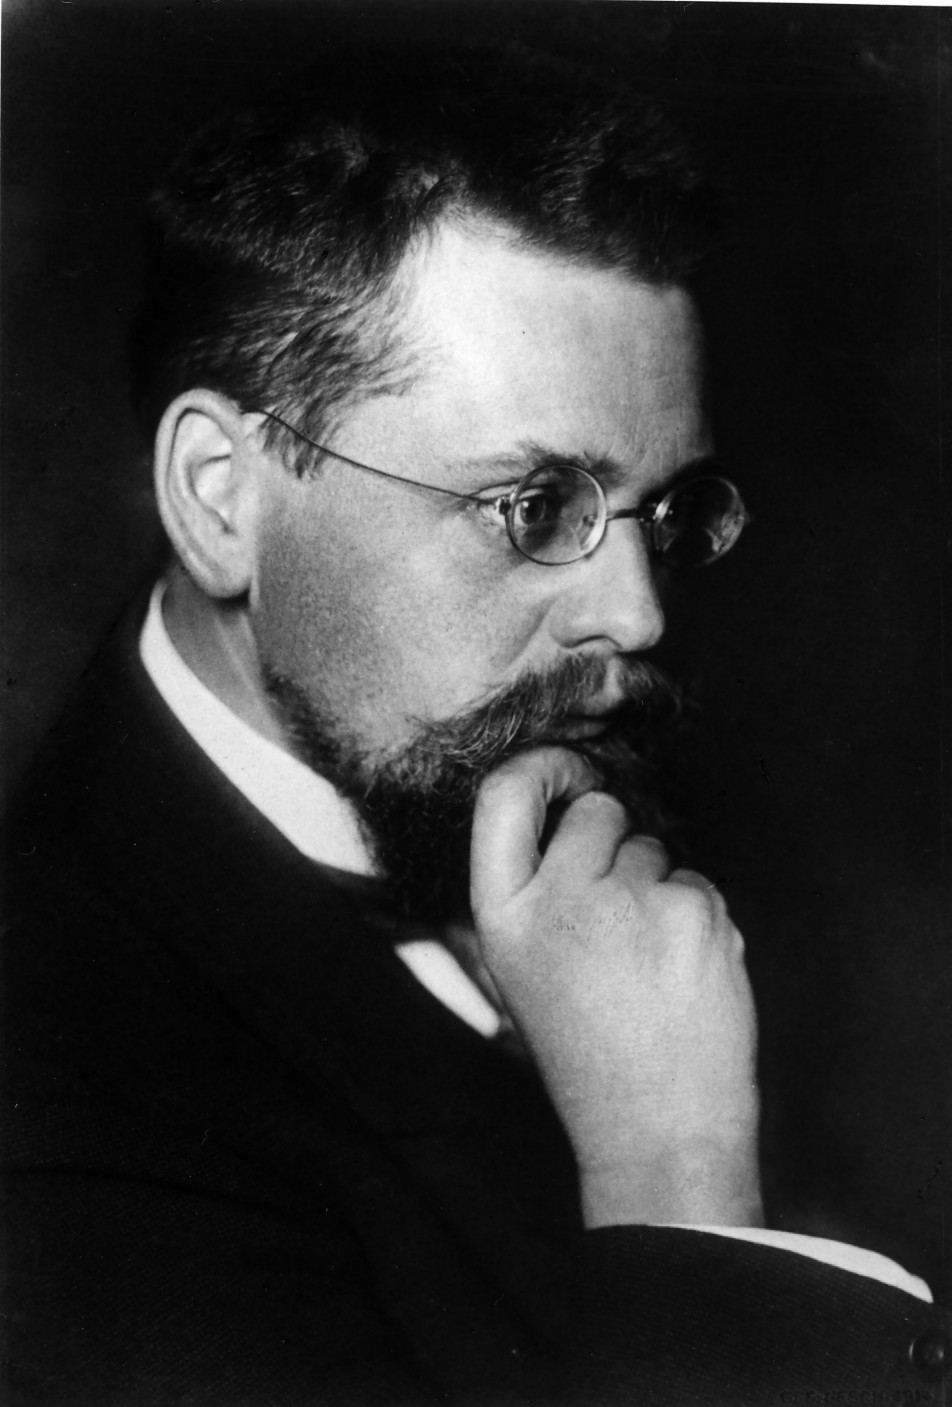
\includegraphics[width=1.5in]{images/PortraitZurich-sw-nb-300.jpg}
	\end{minipage}
	\begin{minipage}{2.25in}
		\centering
		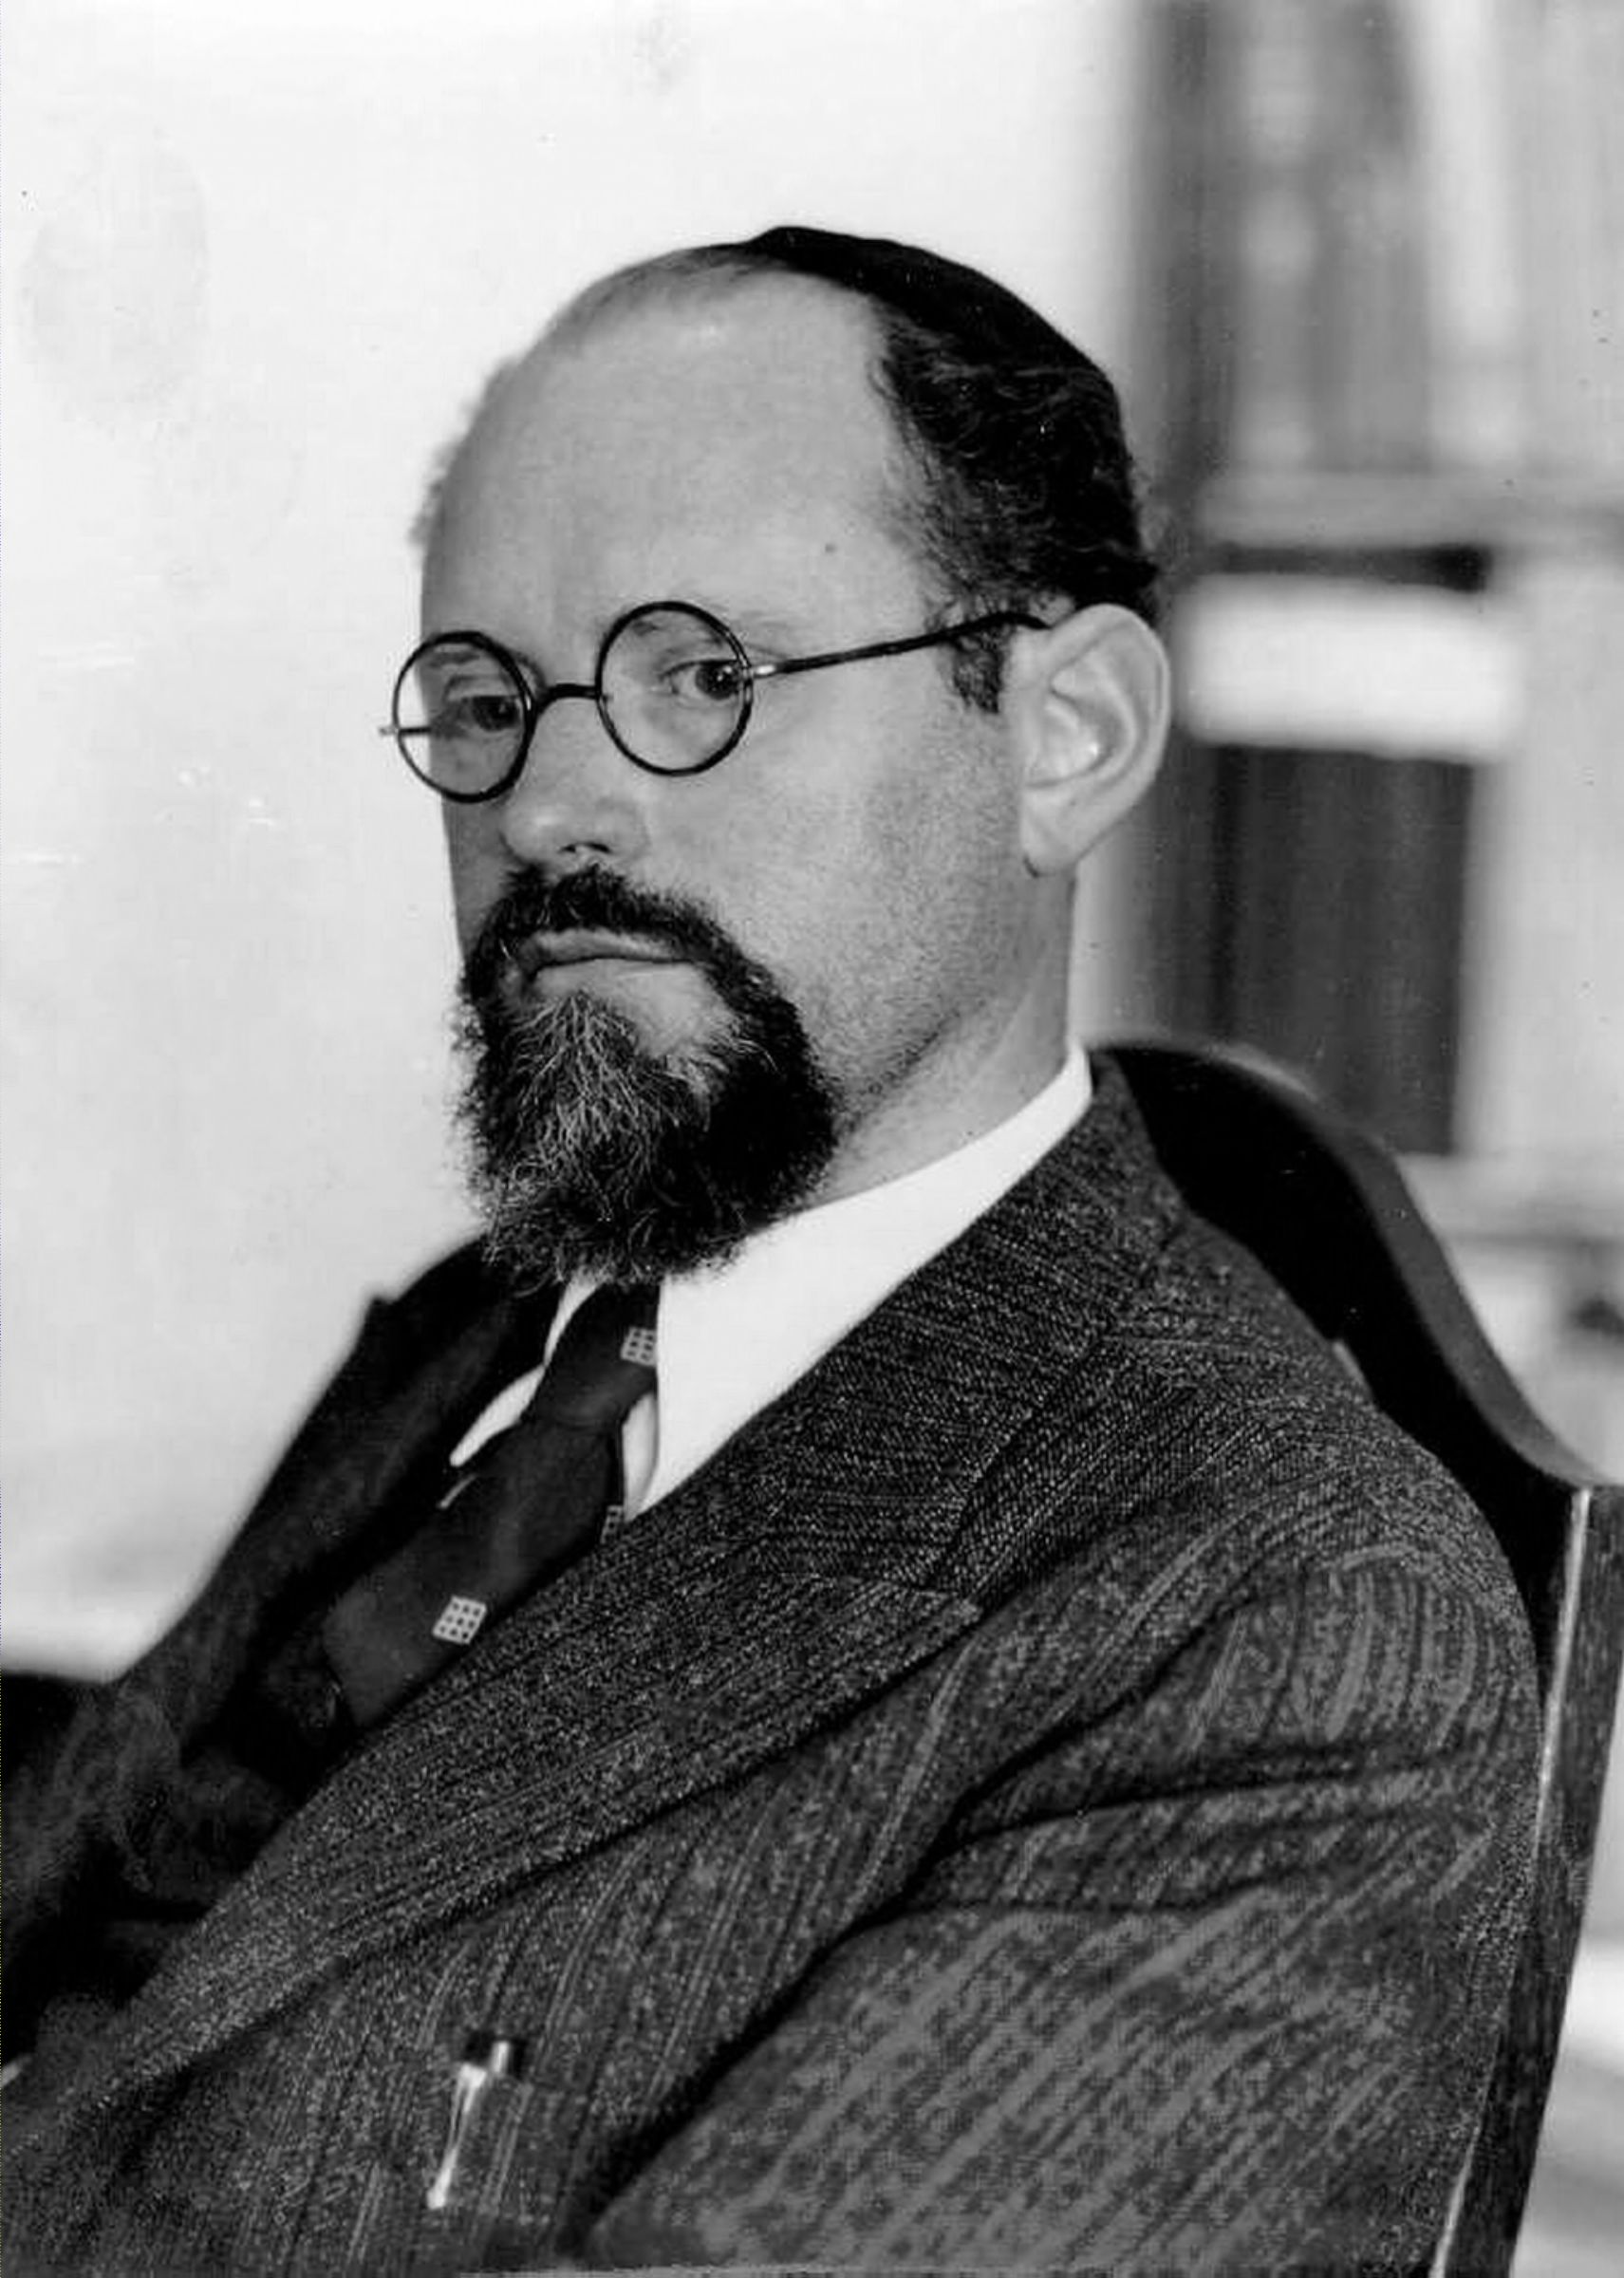
\includegraphics[width=1.75in]{images/Adolf_Abraham_Halevi_Fraenkel.jpg}
	\end{minipage}
	\caption[Ernst Zermelo and Abraham Fraenkel]{Set theorists Ernst Friedrich Ferdinand Zermelo \cite{mildenberger2014}, left; and Abraham Halevi ``Adolf'' Fraenkel \cite{fraenkel-photo}, right.}\label{zfphoto}
\end{figure}
Zermelo--Fraenkel set theory is a theory of well-founded sets named after the German-born set theorists Ernst Zermelo (1871--1953) and Abraham Fraenkel (1891--1965), both of whom are pictured in Figure \ref{zfphoto}. The men went their separate ways.  Zermelo remained at the University of Berlin, where he had received his doctorate in 1894.  Fraenkel was active in the Mizrachi religious Zionist movement \cite{cohen-mansfield2016}, and about the beginning of the Great Depression, he exercised what would later, after the war, become Israel's Law of Return to take a post as the first Dean of Mathematics at the Hebrew University of Jerusalem.
\begin{definition}\label{def-set}
	In this theory, every \textbf{set} is a collection of things, and every thing in existence is a \textbf{set}.
\end{definition}
\begin{definition}
	When a thing $x$ is a \textbf{member} or \textbf{element} of the collection $C$, we use the symbol $\in$, a stylized stick figure of the lower-case Greek letter epsilon,\footnote{Cf.\ elementhood symbol {\huge$\in$}, lower-case epsilon {\huge$\epsilon$}, set in huge type.  This and many other symbols of set theory were invented by Giuseppe Peano \cite{peano1901}, Figure \ref{peanophoto}.} and we write \mbox{$x\in C$}.  Alternatively we may say that the collection $C$ \textbf{includes} the element $x$, and write \mbox{$C\ni x$}.
\end{definition}
\begin{definition}\label{def-well-founded}
	A set $X$ is said to be \textbf{well-founded} if there is \textbf{\textit{no}} infinite descending chain of membership or elementhood from $X$:
	\begin{equation}
	X\ni X_1
	\land X_1\ni X_2
	\land X_2\ni X_3
	\land X_3\ni \cdots\label{idcx}
	\end{equation}
\end{definition}
\begin{remark}
	If there \textit{is} such an infinite descending chain (\ref{idcx}) from $X$, we say that the set $X$ is \textit{ill-founded}.  The axioms of Zermelo--Fraenkel set theory preclude the existence of ill-founded sets.\footnote{Those who tell stories of ``turtles all the way down'' and other New Age nonsense are talking about an ill-founded world.  Those of such beliefs who admit the existence of such sets may study instead Willard Van Orman Quine's New Foundations set theory \cite{sep-quine-nf} which is based on stratified types and does admit ``turtles all the way down.''  Many open questions remain, and although it is now many years old, New Foundations set theory has not yet undergone a sufficient critical assessment to determine its fitness to serve as a foundation for mathematics and computer science.}
\end{remark}
\begin{definition}
	When every thing that is a member of a collection $B$ is also a member of the collection $C$, we write \mbox{$B\subset C$} and say that $B$ \textbf{is contained in} $C$, or that $C$ \textbf{contains} $B$; alternatively we may write \mbox{$C\supset B$}.
\end{definition}
\begin{definition}\label{def-eq}
	We say that the sets $A$ and $B$ are \textbf{equal} and we write $A=B$ if $A\subset B$ and $B\subset A$.
\end{definition}
\begin{definition}
	If $C$ contains $B$, and there exists some member of the collection $C$ that is not a member of the collection $B$, then we say that $C$ \textbf{properly contains}\footnote{Alternatively, ``\textbf{\textit{properly extends}}'' or similar language.} $B$.  This is sometimes written \mbox{$C\supsetneqq B$}, or \mbox{$B\subsetneqq C$}.  $P$ and $NP$ from the title of this paper, but we mention as an example at this point that while we know that $P\subset NP$, the whole $P$ vs.\ $NP$ question rests on whether or not $NP$ properly contains $P$.
\end{definition}
\begin{remark}
	If a set $A$ is contained in the set $B$, then $A$ is either equal to $B$ or properly contained in $B$:
	\begin{equation}
	A\subset B\longrightarrow A=B\lor A\subsetneqq B.
	\end{equation}
	The entire $P$ vs.\ $NP$ question is the question of whether \mbox{$P=NP$} or \mbox{$P\subsetneqq NP$}, since we know that \mbox{$P\subset NP$}. 
\end{remark}
\subsection{Language of set theory}
\begin{table}
\begin{bnf*}
	\bnfprod{wff}
		{\bnfpn{f5}}\\
	\bnfprod{f5}
		{\bnfpn{f4}\bnfor\bnfpn{f4}\longleftrightarrow\bnfpn{f4}}\\
	\bnfprod{f4}	
		{\bnfpn{f3}\bnfor\bnfpn{f4}\longleftarrow\bnfpn{f3}}\\
	\bnfprod{f3}
		{\bnfpn{f2} \bnfor \bnfpn{f2} \longrightarrow \bnfpn{f3}}\\
	\bnfprod{f2}
		{\bnfpn{f1} \bnfor \bnfpn{f2} \lor \bnfpn{f1}}\\		
	\bnfprod{f1}
		{\bnfpn{f0} \bnfor \bnfpn{f1} \land \bnfpn{f0}}\\
	\bnfprod{f0}\label{fprod}
		{\bnfpn{set}\bnfpn{b}\bnfpn{set}
		\bnfor \lnot\bnfpn{f0}
		\bnfor (\bnfpn{wff})}\\
	&&{	\bnfor (\exists\bnfpn{var})\bnfpn{f0}
		\bnfor (\forall\bnfpn{var})\bnfpn{f0}
		\bnfor \top \bnfor \bot
		}\\
	\bnfprod{set}
		{\bnfpn{s5}}\\
	\bnfprod{s5}
		{\bnfpn{s4}\bnfor\bnfpn{s4}\,\backslash\,\bnfpn{s5}}\\
	\bnfprod{s4}
		{\bnfpn{s3}\bnfor\bnfpn{s4}\,\triangle\,\bnfpn{s3}}\\
	\bnfprod{s3}
		{\bnfpn{s2}\bnfor\bnfpn{s3}\,\cup\,\bnfpn{s2}}\\
	\bnfprod{s2}
		{\bnfpn{s1}\bnfor\bnfpn{s2}\,\cap\,\bnfpn{s1}}\\
	\bnfprod{s1}
		{\bnfpn{s0}\bnfor\bnfpn{s1}\times\bnfpn{s0}\\}
	\bnfprod{s0}
		{\bnfpn{var}\bnfor\bigcup\bnfpn{s0}\bnfor\{\bnfpn{ss}\}\bnfor(\bnfpn{ss})}\\
	&&{\bnfor\{\bnfpn{var}\in\bnfpn{set}|\bnfpn{wff}\}}\\
	\bnfprod{ss}
		{\bnfpn{set}\bnfor\bnfpn{ss},\bnfpn{set}}\\
	\bnfprod{b}
		{\in \bnfor \notin \bnfor \ni \bnfor \not\ni
			\bnfor \subset \bnfor \not\subset
			\bnfor \supset \bnfor \not\supset
			\bnfor = \bnfor \neq
			\bnfor \subsetneqq \bnfor \supsetneqq}\\
	\bnfprod{var}\label{varprod}
		{\textit{A}\bnfsk\textit{Z}
		\bnfor \textit{a}\bnfsk\textit{z}
		\bnfor \alpha \bnfsk \omega
		\bnfor \bnfsk}
\end{bnf*}
\caption{Context-free grammar for set theory}\label{settheorygrammar}
\end{table}

\begin{definition}
A \textbf{well-formed formula} is best defined in Backus--Naur form as a context-free grammar as in Grammar~\ref{settheorygrammar}.

Beginning from the initial symbol $\bnfpn{wff}$, productions are carried out by replacing a symbol to the left of ``$\bnfpo$'' by one of the alternatives (sequences or strings of symbols) listed on the right, separated by vertical bars.  Those symbols enclosed by angle brackets $\bnfpn{\dots}$ are non-terminal, and production must continue until all non-terminal symbols have been replaced by literal non-bracketed terminal symbols.


Whenever a well-formed formula is generated by Grammar~\ref{settheorygrammar}, rules for the scoping of variables ``$\bnfpn{var}$'' must be applied as expressions are generated by this grammar, in particular with respect to the ``binding'' productions
$(\exists\bnfpn{var})\bnfpn{f}$, 
$(\forall\bnfpn{var})\bnfpn{f}$, and
$\{\bnfpn{var}\in\bnfpn{set}\,|\,\bnfpn{wff}\}$,
Any free variable $\bnfpn{var}$ occurring in a formula $\bnfpn{f}$ or $\bnfpn{wff}$ is considered to remain free until it is bound by the explicit use of an existential $(\exists\cdots)$ or universal $(\forall\cdots)$ quantifier or set-builder $\{\cdots\in\cdots\,|\,\cdots\}$ notation.  A well-formed formula may be denoted at a more abstract ``meta'' level by a greek letter followed by its list of free variables (if any) in parentheses, e.g. $\varphi(x,y,z)$.

The major significance of the concept of ``well-formed formula'' is that such formulas are non-trivial to define, and the axiom schemata of Zermelo--Fraenkel set theory do depend on such a rigorous definition.  We do not propose at this time that Grammar~\ref{settheorygrammar} is complete or correct or that it corresponds to common or accepted usage.
\end{definition}
\begin{definition}
The main \textbf{verbs} of the language of set theory are defined here. 
\begin{align}
X\in Y \quad&\longleftrightarrow\quad \textrm{``\textit{X} is an element of \textit{Y}.''}\\
X\notin Y \quad&\longleftrightarrow\quad \textrm{``\textit{X} is not an element of \textit{Y}.''}\\
X\ni Y \quad&\longleftrightarrow\quad \textrm{``\textit{X} includes (as an element) \textit{Y}.''}\\
X\not\ni Y \quad&\longleftrightarrow\quad \textrm{``\textit{X} does not include \textit{Y}.''}\\
X\subset Y \quad&\longleftrightarrow\quad \textrm{``\textit{X} is contained in \textit{Y}.''}\\
X\not\subset Y \quad&\longleftrightarrow\quad \textrm{``\textit{X} is not contained in \textit{Y}.''}\\
X\supset Y \quad&\longleftrightarrow\quad \textrm{``\textit{X} contains \textit{Y}.''}\\
X\not\supset Y \quad&\longleftrightarrow\quad \textrm{``\textit{X} does not contain \textit{Y}.''}\\
X=Y \quad&\longleftrightarrow\quad \textrm{``\textit{X} equals \textit{Y}.''}\\
X\ne Y \quad&\longleftrightarrow\quad \textrm{``\textit{X} does not equal \textit{Y}.''}\\
X\subsetneqq Y \quad&\longleftrightarrow\quad \textrm{``\textit{X} is properly contained in \textit{Y}.''}\\
X\supsetneqq Y \quad&\longleftrightarrow\quad \textrm{``\textit{X} properly contains \textit{Y}.''}
\end{align}
\end{definition}
\begin{definition}
The \textbf{binary set operations} of \textbf{intersection} (\ref{def-n}), union (\ref{def-u}), \textbf{difference} (\ref{def-diff}), \textbf{discrepancy} or \textbf{symmetric difference} (\ref{def-disc}), and \textbf{Cartesian product} (\ref{def-cart-prod}) are defined.
\begin{align}
	X\cap Y&=\{x\in X|x\in Y\};\label{def-n}\\
	X\cup Y&=\bigcup\{X,Y\};\label{def-u}\\
	X\operatorname{\backslash}Y&=\{x\in X|x\notin Y\};\label{def-diff}\\
	X\operatorname{\triangle}Y&=(X\operatorname{\backslash}Y)\cup(Y\operatorname{\backslash}X);\label{def-disc}\\
	X\times Y
	&=
	\left\{
		p\in\mathscr P\big(\mathscr P(X\cup Y)\big)
		\left|
			\begin{array}{r}(\exists y)\\(\exists x)\end{array}\left(\begin{array}{r}\big\{\{x\},\{x,y\}\big\}=p\\\land\, x\in X \land y\in Y\end{array}\right)
		\right.
	\right\}.\label{def-cart-prod}
\end{align}
\end{definition}


\subsection{Basic axioms}\label{sect-zf-axioms}
\begin{definition}
	The symbol $\exists$, an upside-down stick figure of the upper-case letter `E,' is called the \textbf{existential quantifier}, and it is used to assert the existence of some thing satisfying the  formula immediately following.
\end{definition}
\begin{definition}
	The symbol $\forall$, an upside-down stick figure of the upper-case letter `A,' is called the \textbf{universal quantifier}, and it is used to make a statement that every thing in existence satisfies the formula immediately following. 
\end{definition}
\begin{axiom}[Power Set]\label{powerset}
	For any given set $q$, there is a set $p$ such that every subset of $q$ is an element of $p$.
	\begin{equation}
	(\forall q)(\exists p)(\forall s)(s\subset q\longrightarrow s\in p).
	\end{equation}
\end{axiom}
\begin{axiom}[Union]\label{unionset}
	If $w$ is a set, then there exists a set $u$ including all elements of elements of $w$.
	\begin{equation}
	(\forall w)(\exists u)(\forall z)\,\big(z\in u\longleftarrow(\exists x)(z\in x\land x\in w)\big).
	\end{equation}
\end{axiom}
\begin{axiom}[Infinity] \label{infinityset}
	There exists a non-empty set $\omega$ including, for every set $\alpha$, also a set $\beta$, being a proper superset of $\alpha$:
	\begin{equation}
	(\exists \omega)\bigg((\exists \alpha)\, \alpha\in \omega\land (\forall \alpha)\big(\alpha\in \omega\longrightarrow (\exists\beta)(\beta\in\omega\land\beta\supsetneqq\alpha)\big)\bigg)
	\end{equation}
\end{axiom}
\subsection{Axiom schemata}\label{zf-sect-schemata}
\textbf{ZF} set theory is not finitely axiomatizable.  It requires certain \textit{schemata}, which may not be used as such in a proof, but must be \textit{instantiated} on an arbitrary well-formed formula.  These statements are considered valid of any well-formed formula, but an axiom schema may not be used in a proof unless it is instantiated upon a particular well-formed formula.

Basically, \textbf{Tarski's theorem on the undefinability of truth} prevents us from quantifying universally or existentially with respect to truth value, in any formal system capable of adequate arithmetic, over arbitrary well-formed formulas of that same system.\footnote{In order to express such a quantification on arbitrary formulas, we must strictly bound the number of alternations of quantification (between universal and existential) in the formula, express the formula in prenex form, and then quantify literally over the rudimentary part of the formula. Thus we may make statements of $\Sigma_1$-soundness, $\Sigma_2$-soundness, etc., but we may not make, within any sound formal system, an unbounded statement of the soundness of that system.}

\begin{axiomschema}[Comprehension]\label{comprehensionschema}
	Let $\varphi(x)$ be a well-formed formula. Then for any set $t$ there is a set $s$ including exactly those elements $x$ of $t$ such that $\varphi(x)$ is true; i.e.,
	\begin{equation}
	[\textrm{wff }\varphi(x)]\qquad(\forall t)(\exists t)(\forall x)\big(x\in s\longleftrightarrow x\in t\land\varphi(x)\big).
	\end{equation}
\end{axiomschema}
\begin{axiomschema}[Replacement]\label{replacementschema}
	Let $\varphi(x,y)$ be a well-formed formula.  If $w$ is a set and for every element $x$ of $w$ there exists $y$ satisfying $\varphi(x,y)$, then there exists a set $z$ including as an element such $y$ for every element $x$ of $w$.
	\begin{equation}
	\begin{array}{rl}
	[\textrm{wff }\varphi(x,y)]
	& (\forall w)\Big((\forall x)(x\in w\longrightarrow(\exists y)\varphi(x,y)) \\
	&\qquad	\longrightarrow (\exists z)(\forall x)\big(x\in w\longrightarrow (\exists y)(y\in z\land\varphi(x,y))\big)\Big).
	\end{array}
	\end{equation}
\end{axiomschema}
\begin{axiomschema}[Regularity]\label{regularityschema}
	Let $\varphi(x)$ be a well-formed formula expressing some property of the arbitrary set $x$.  If this property be true of the arbitrary set $y$ whenever it is true of all the elements $x$ of $y$, then it is true of all sets $x$.
	\begin{equation}
	[\textrm{wff }\varphi(x)]\qquad (\forall y)\big((\forall x)(x\in y\longrightarrow\varphi(x))\longrightarrow\varphi(y)\big)\longrightarrow(\forall x)\varphi(x).
	\end{equation}
\end{axiomschema}
\begin{remark}
	The axiom schema of regularity is a principle of induction on the well-foundedness of sets.
\end{remark}
\begin{definition}\label{def-zf}
	\textbf{ZF} is the system of axioms \Axiom\ref{emptyset}, \Axiom\ref{powerset}, \Axiom\ref{pair}, \Axiom\ref{unionset}, \Axiom\ref{infinityset}, \AxiomSchema\ref{comprehensionschema}, \AxiomSchema\ref{replacementschema}, and \AxiomSchema\ref{regularityschema}.
\end{definition}
\subsection{Basic theorems of \textbf{ZF}}
\begin{theorem}[Empty set]\label{emptyset}
	There exists a set $X$ such that for every thing $Y$, $Y$ is not an element of $X$.  In symbols we write this,
	\begin{equation}
	(\exists X)(\forall Y)\;Y\notin X.
	\end{equation}
\end{theorem}
\begin{proof}
	Empty set is an instance of the schema \AxiomSchema\ref{comprehensionschema} on any self-contradictory or always-false well-formed formula,
	with any set already postulated to exist, say, by \Axiom \ref{infinityset}; comprehending those elements of that set (namely none of them) that satisfy the always-false formula.
\end{proof}
\begin{theorem}[Pair]\label{pair}
	If $X$ is a set and $Y$ is a set, then a set $W$ exists, such that \mbox{$Z\in W$} if and only if \mbox{$Z=X$} or \mbox{$Z=Y$}.
	\begin{equation}\label{eq-pair}
	(\forall X)(\forall Y)(\exists W)(\forall Z)(Z\in W\longleftrightarrow Z=X\lor Z=Y).
	\end{equation}
\end{theorem}
\begin{proof}
	Pair is an instance of replacement \AxiomSchema\ref{replacementschema} on any set having at least two elements already postulated to exist, say, by infinity \Axiom\ref{infinityset}.
\end{proof}
\begin{theorem}[Ordered pair]
	There is a well-formed formula $\Omega_2(x,y,z)$ allowing a particular set $z$ to represent the \textbf{ordered pair} $(x,y)$.  In particular, for all sets $x$ and $y$, there is a set $z$ satisfying $\Omega_2(x,y,z)$, and if $\Omega_2(x,y,z)$ and $\Omega_2(x,y,w)$, then $w=z$  Conversely for all sets $u$ and $v$, $u=x$ and $v=y$ if and only if $\Omega_2(x,y,z)$ and $\Omega_2(u,v,z)$.
	\begin{equation}
		\begin{array}{r}(\forall x)\\(\forall y)\end{array}
		\left(\begin{array}{rl}
			(\exists z)&\big(\Omega_2(x,y,z)\big)\\
			&\land\\
			\begin{array}{r}(\forall z)\\(\forall w)\end{array}&
				\left(\begin{array}{c}(\Omega_2(x,y,z)\land\Omega_2(x,y,w)\longrightarrow w=z)\\
			\land\\
			(\Omega_2(x,y,z)\land\Omega_2(u,v,z)\longleftrightarrow u=x		
			\land v=y)\end{array}\right)
		\end{array}\right)
	\end{equation}
\end{theorem}
\begin{proof}
Set
	\begin{equation}
		\Omega_2(x,y,z) \longleftrightarrow z=\big\{\{x\},\{x,y\}\big\}.
	\end{equation}
Then, for any $z$, if $(\exists x)(\exists y)\Omega_2(x,y,z)$, then
	\begin{align}
		x &= \bigcup \bigcap z;\label{pair1st}\\
		y &= \bigcup \bigcap \left(\left\{\bigcup z\operatorname{\backslash}\bigcup z,\bigcap z\right\}\operatorname{\backslash}\{\emptyset\}\right).\label{pair2nd}
	\end{align}
	The first element of the pair (\ref{pair1st}) is trivial. The extraction of the second element of the ordered pair (\ref{pair2nd}) is somewhat more complicated.
	\begin{equation}
	\bigcup z \operatorname{\backslash}\bigcap z = \left\{\begin{array}{cr}
	\{y\},&x\ne y;\\\emptyset,&x=y.
	\end{array}\right.
	\end{equation}
	Now we have
	\begin{equation}
	\left\{\bigcup z\operatorname{\backslash}\bigcup z, \bigcap z\right\}\operatorname{\backslash}\{\emptyset\} = \{\{y\},\{x,y\}\},
	\end{equation}
	which is the reverse of the original ordered pair $(x,y)$, so in (\ref{pair2nd}) we extract the first element of $(y,x)$ with the same operation that we used in (\ref{pair1st}).
\end{proof}
\subsection{Axiom of choice}
\begin{axiom}[Choice]\label{axiomchoice}
	If $B$ is a set, no element of $B$ is empty, and no two elements of $B$ include the same set as an element, then there exists a ``choice'' set $C$ including one and only one element of each element of $B$.
	\begin{equation}
	(\forall B)\left(\begin{array}{l}\begin{array}{l}
	\begin{array}{c}
	(\forall b)\big(b\in B\longrightarrow(\exists x)x\in b\big)\\
	\land\\(\forall b_1)(\forall b_0)
	\left(\begin{array}{l}
	b_0\in B\land b_1\in B\\
	\quad\longrightarrow(b_1\ne b_0\longrightarrow b_0\cap b_1=\emptyset)\end{array}\right)\end{array}\\~\\
	\end{array}\\
	\longrightarrow\\\quad
	(\exists C)\left(\begin{array}{c}
	(\forall b)
	\left(\begin{array}{l}
	b\in B\\
	\longrightarrow(\exists c)(c\in C\land c\in b)\\
	\end{array}
	\right)\\
	\land\\
	\begin{array}{r}
	(\forall c_1)\\(\forall c_0)\\
	(\forall b_1)\\(\forall b_0)\\
	\end{array}
	\left(
	\begin{array}{l}
	b_0\in B\land b_1\in B\\
	\quad\land\, c_0\in C\land c_1\in C\\
	\quad\land\, c_0\in b_0 \land c_1\in b_1\\
	\longrightarrow (c_1\ne c_0\longrightarrow b_1\ne b_0)
	\end{array}
	\right)
	\end{array}\right)
	\end{array}\right)\label{choice-eqn}
	\end{equation}
\end{axiom}
\begin{remark}
	The statement (\ref{choice-eqn}) is artistically arranged but intended to conform to the rules of Grammar~\ref{settheorygrammar}.  The exercise of constructing it reveals a certain awkwardness in the grammar, because only unrestricted quantification is specified (\ref{fprod}), which requires a circumlocution $(\forall b)(b\in B\longrightarrow\cdots)$ to express the restricted quantification $(\forall b\in B)\cdots$.
	
	There are numerous alternative formulations of the axiom of choice and it is an interesting and instruction exercise to prove that these are all equivalent.  One alternative states the existence of a ``choice function'' rather than a ``choice set'' as we have done above, but this is less elementary as it depends on the precise definition of ``function'' from that of ``ordered pair.''  Another important alternative is the statement ``Every set may be well-ordered.''
\end{remark}
	The axiom of choice is independent\footnote{Cohen discovered that the axiom of choice cannot be proven from the other axioms unless those axioms themselves are inconsistent.}  and may be considered optional.	
\begin{definition}
	\textbf{ZFC} is the system of axioms \textbf{ZF} together with \Axiom \ref{axiomchoice}.
\end{definition}
\subsection{Classes}
One may remark on the presence of \AxiomSchema\AxiomSchema \ref{comprehensionschema}, \ref{replacementschema}, \ref{regularityschema}; \textbf{ZF} set theory is not finitely axiomatizable.  However, there is a conservative extension of it, \textbf{NBG} or von-Neumann--G{\"o}del--Bernays set theory, which is finitely axiomatizable without schemata, and still able to prove all the theorems provable in \textbf{ZF}.  This depends on introducing the concept of a \textbf{proper class}, capable of including elements as a set, but itself incapable of elementhood; a proper class is considered ``too big'' to be a set.  Little is lost, however, as there are circumlocutions in \textbf{ZF} set theory to speak of proper classes.
\begin{circumlocution}
	For any well-formed formula $\varphi(x)$, we may speak of the \textbf{class} of all sets $x$ that satisfy $\varphi(x)$.  If, for example, we name this class $\mathbf{X}$, we may write
	\begin{equation}
	(\forall x)(x\in\mathbf X \longleftrightarrow \varphi(x)).
	\end{equation}
	However we cannot say on this basis alone in Zermelo--Fraenkel set theory that $\mathbf X$ ``exists'' or that $\mathbf X$ is a set by \Definition \ref{def-set}.  The Axiom Schema of Comprehension \AxiomSchema \ref{comprehensionschema} can only make a set of those $x$ satisfying $\varphi(x)$ \textit{which are already elements of some pre-existing \textbf{set} $Z$}.
\end{circumlocution}
\begin{remark}
	Every element of a class, necessarily, is a set.
\end{remark}
\begin{circumlocution}
	If $\mathbf X=\{x\,|\,\varphi(x)\}$ is a class, and
	\begin{equation}
	(\forall Z)(\exists x)(x\in\mathbf X\land x\notin Z),
	\end{equation}
	i.e.\
	\begin{equation}
	(\forall Z)(\exists x)(\varphi(x)\land x\notin Z),	
	\end{equation}
	then $\mathbf X$ is said to be a \textbf{proper class}.  Otherwise,
	if
	\begin{equation}
	(\exists Z)(\forall x)(x\in\mathbf X\longrightarrow x\in Z),
	\end{equation}
	i.e.\
	\begin{equation}
	(\exists Z)(\forall x)(\varphi(x)\longrightarrow x\in Z),
	\end{equation}
	then $\mathbf X$ is said to be a \textbf{small class}, because it satisfies the criteria of \AxiomSchema \ref{comprehensionschema} to be a set.
\end{circumlocution}
\begin{remark}
No proper class is
\begin{itemize}
	\item a set;
	\item an element of a set; or,
	\item a subset of a set.
\end{itemize}
It is for this reason that proper classes are sometimes said to be ``too big'' to be sets.
\end{remark}
\section{Peano arithmetic}\label{sect-pa}
\begin{figure}
	\centering
	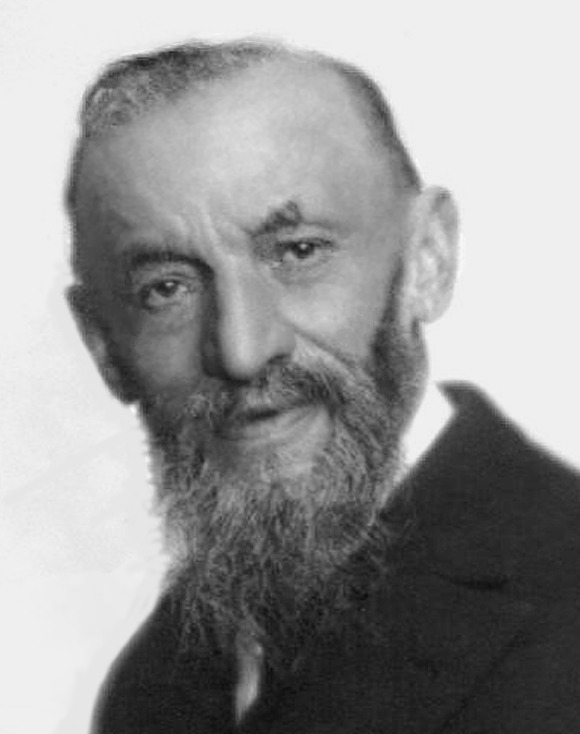
\includegraphics[width=1.5in]{images/Giuseppe_Peano.jpg}
	\caption[Giuseppe Peano]{~\\Italian mathematician Giuseppe Peano \cite{peano-photo},\\godfather of ``Peano arithmetic.''}
	\label{peanophoto}
\end{figure}
\subsection{Introduction}
Up to a certain point we have worked with the notion of provability in some vague, indefinite formal system $F$.  We have come to the realization that without enumerating the axioms of the system $F$ or specifying it any further, we cannot hope to show that some statement such as $P=NP$ or $P\ne NP$ is independent of those axioms; otherwise we could just as well show the same statement to be independent of the systems $F+[P=NP]$ and $F+[P\ne NP]$ \cite{spector2016ans}.

This brings us to consider the system of arithmetic named after the Italian mathematician Giuseppe Peano (1858--1932) [Figure~\ref{peanophoto}].
\subsection{Axioms}
The axioms of this system are five in number \cite[p.~149]{haowang1957}, or rather, four plus an axiom schema valid for any predicate or propositional function.

\begin{axiom}\label{p1}
	$(\exists n)\,n=1$.
\end{axiom}
\begin{axiom}\label{p2}
	$(\forall m)(\exists n)\,n=m+1$.
\end{axiom}
\begin{axiom}\label{p3}
	$(\forall m)(\forall n)\,(n\ne m\longrightarrow n+1\ne m+1)$
\end{axiom}
\begin{axiom}\label{p4}
	$(\forall n)\,n+1\ne 1$.
\end{axiom}
\begin{axiomschema}\label{p5}
	For any predicate or propositional function $\varphi(n)$,
	\begin{equation}
	\varphi(1)\land(\forall n)\,\big(\varphi(n)\longrightarrow\varphi(n+1)\big)\longrightarrow(\forall n)\,\varphi(n)
	\end{equation}
	is an axiom.
\end{axiomschema}


There seems to be a great deal of popular confusion regarding Axiom Schema \ref{p5}.  It was never intended to be universally quantified in some indefinite sense to make second-order statements.  Such an axiom schema must be fully instantiated every time it is used in a proof, and no statement should be considered provable from the axioms of Peano arithmetic unless it can be validly deduced in a finite number of steps from \Axiom\Axiom \ref{p1}--\ref{p4} and a necessarily finite number of full, complete instantiations of \AxiomSchema \ref{p5}.
\begin{remark}
Programmers might find a vague analogy between an axiom schema and a \texttt{template} in C++ \cite{cpptemplate}.  Addition, comparison, and multiplication are not axioms in Peano arithmetic, but their definitions (to follow) are justified by Axiom Schema~\ref{p5}.
\end{remark}

\begin{definition}
	\textbf{Addition} in Peano arithmetic is defined for any number $m$ by repeating the ``successor'' operation which we have denoted ``$+1$.''
	\begin{itemize}
		\item $m+1$ behaves as laid out in \Axiom\Axiom \ref{p1}--\ref{p4} and \AxiomSchema\ref{p5}.
		\item $(\forall n)\,m+(n+1)=(m+n)+1$.
	\end{itemize}
	The term to the left of the ``$+$'' sign is called the \textbf{augend}, and the term to the right is called the \textbf{addend}.  The result of this operation is called the \textbf{sum}.
\end{definition}
\begin{remark}
	The augend is understood to be number that is ``augmented,'' increased, or operated on by the addition, and the addend is the number being added to it. Addition is commutative, and Peano arithmetic only speaks of positive numbers; but the distinction is nonetheless important from a foundational point of view, and made a little more clear by analogy to subtraction, where the \textit{minuend} is the number being ``diminished'' or operated on by the subtraction and the \textit{subtrahend} is the number being subtracted from it to obtain the \textit{difference}.
\end{remark}
\begin{definition}
	\textbf{Strict comparison} of any numbers $m$ and $n$ in Peano arithmetic is defined by the existence of a positive difference $d$.
	\begin{itemize}
		\item $m<n\quad\longleftrightarrow\quad (\exists d)\,m+d=n$.
		\item $m>n\quad\longleftrightarrow\quad (\exists d)\,m=n+d$.	
	\end{itemize}
	When $m<n$, we say that $m$ is \textbf{less than} $n$ or that $m$ is \textbf{the lesser} of the two numbers $m$ and $n$.  When $m>n$, we say that $m$ is \textbf{greater than} $n$, or that $m$ is \textbf{the greater} of the two numbers $m$ and $n$.
\end{definition}

\begin{definition}
	\textbf{Loose comparison} is defined by logical disjunction with equality, where equality behaves as enumerated in \Axiom\Axiom \ref{p1}--\ref{p5}.
	\begin{itemize}
		\item $m\leqq n\quad\longleftrightarrow\quad m<n\lor m=n$.
		\item $m\geqq n\quad\longleftrightarrow\quad m>n\lor m=n$.	
	\end{itemize}
When $m\leqq n$, we say that $m$ is \textbf{less than or equal to} $n$.  When $m\geqq n$, we say that $m$ is \textbf{greater than or equal to} $n$.
\end{definition}

\begin{definition}
	\textbf{Multiplication} in Peano arithmetic is defined for any number $n$ by repeated addition.
	\begin{itemize}
		\item $1n=n$.
		\item $(\forall m)\,(m+1)n=mn+n$.
	\end{itemize}
	The factor juxtaposed on the left is called the \textbf{multiplier} and the factor to the right is called the \textbf{multiplicand}.  The result of this operation is called the \textbf{product}.
\end{definition}
\begin{remark}	
	Multiplication, too, is commutative in Peano artihmetic, but it is nonetheless important from a foundational point of view to distinguish between the factors: the multiplicand is understood to be the number being operated on, in this case being multiplied, whereas the multiplier specifies how many ``times'' it is being multiplied, or repeatedly added.
\end{remark}

\begin{theorem}Peano arithmetic may be interpreted in Zermelo--Fraenkel set theory.
\end{theorem}
\begin{proof}
	The strategy of this proof is very simple, straighforward, and mechanical, though perhaps a bit tedious.  We set our universe of discourse for Peano arithmetic to be the set of non-empty elements of $\omega_0$, that is, the set $\mathbb N=\omega_0\operatorname{\backslash}\{\emptyset\}$ in Zermelo--Fraenkel theory.  Then we prove, in \textbf{ZF}, that the set $\mathbb N$ satisfies all the axioms of Peano arithmetic.  The successor operation in \textbf{PA}, $n\longmapsto n+1$, is translated to a union with the singleton including set in \textbf{ZF}: $n\longmapsto n\cup\{n\}$.
	\begin{enumerate}
		\item [\Bearing\ref{p1}.] The number one is translated to the set including just the empty set:
		\begin{equation}
		(\exists n)\,n\in\mathbb N\land n=\{\emptyset\}.
		\end{equation}
		\item [\Bearing\ref{p2}.] The ``successor'' operation which we have denoted ``$+1$'' in Peano arithmetic is translated to the operation described in \textbf{ZF}'s Axiom of Infinity \ref{infinityset}:
		\begin{equation}
		(\forall m)(m\in\mathbb N\longrightarrow(\exists n)\,n\in\mathbb N\land n=m\cup\{m\}).
		\end{equation}
		\item [\Bearing\ref{p3}.] The axiom that different numbers have different successors may be translated into \textbf{ZF} as
		\begin{equation}(\forall m)(\forall n)\big(m\in\mathbb N\land n\in\mathbb N\land n\ne m\longrightarrow n\cup\{n\}\ne m\cup\{m\}\big).
		\end{equation}
		Its proof follows mechanically from \Definition\ref{def-eq} and from the fact that no well-founded set $n$ (\Definition\ref{def-well-founded}) includes as an element a set including $n$, by virtue of Axiom Schema~\ref{regularityschema}.
		\item [\Bearing\ref{p4}.] Certainly in \textbf{ZF}, $\emptyset\notin\mathbb N$.  If a set $n$ is not the empty set, ...
		\begin{equation}
		(\forall n)\big(n\in\mathbb N\longrightarrow n\cup\{n\}\ne\{\emptyset\}\big).
		\end{equation}
		\item [\LooseBearing\ref{p5}.]  For this we need to strengthen the premise of the induction.  For any given predicate $\varphi(n)$ in Peano arithmetic, consider the predicate $\varphi'(n)$:
		\begin{equation}
		\varphi'(n)\quad\longleftrightarrow\quad(\forall m)\big(m\leqq n\longrightarrow\varphi(m)\big).
		\end{equation}
		Clearly
		\begin{equation}
		(\forall n)\,\varphi'(n)\quad\longleftrightarrow\quad(\forall n)\,\varphi(n),
		\end{equation}
		and thus the principle of induction in Peano artihmetic may be restated in strong form so as for any predicate $\varphi(n)$, 
		\begin{equation}
			(\forall n)\Big((\forall m)\big(m< n\longrightarrow\varphi(m)\big)\longrightarrow\varphi(n)\Big)\quad\longrightarrow\quad(\forall n)\,\varphi(n).
		\end{equation}
		This strong form of induction translates over directly to regularity \ref{regularityschema} because the relation ``$<$'' on the natural numbers in \textbf{PA} translates directly to the relation ``$\in$'' restricted to the set $\omega_0\operatorname{\backslash}\{\emptyset\}$ in \textbf{ZF}.
	\end{enumerate}
	Thus every axiom of Peano arithmetic is ``proven'' in Zermelo--Fraenkel set theory, so that every logical consequence of those axioms is also provable as it is interpreted in \textbf{ZF}.
\end{proof}
\begin{theorem}[Paris--Harrington]
	Peano arithmetic is incomplete with respect to Zermelo--Fraenkel set theory.
\end{theorem}
\begin{proof}
	By this we mean that, unless Peano arithmetic is inconsistent, there are theorems about the natural numbers $\mathbb N$, expressible in the language of Peano arithmetic and provable in Zermelo--Fraenkel set theory, yet not provable in Peano arithmetic itself.
	
	A certain theorem of graph theory, namely the \textbf{\textit{strengthened} finite Ramsey theorem}, is one such theorem \cite{twer1981,ph1,paris1978}.
\end{proof}
\begin{remark}
In increasing order of consistency strength we have Robinson arithmetic $\mathbf Q$, primitive recursive arithmetic $\mathbf{PRA}$, Peano arithmetic $\mathbf{PA}$,  and Zermelo--Fraenkel set theory $\mathbf{ZF}$.  {\color{red}\textbf{???}} The relative strength of Quine's New Foundations theory $\mathbf{NF}$ seems to be unknown.
\end{remark}
\section{Propositional logic: Rules of inference}
\begin{table}[p]
	\centering
	\resizebox{\textwidth}{!}{
\begin{tabular}{|c|c|c|c|c|c|}
	\hline&&&&&\\
	Operation & Symbol & Name & Type & Indroduction & Elimination 
	\\&&&&&\\\hline\hline&&&&&\\
	Verum & $\top$ & true & null
	& $\dfrac{\textrm{(cælum)}}{\top}$ & $\dfrac{\top\longrightarrow p}{p}$
	\\&&&&&\\\hline&&&&&\\
	Falsum & $\bot$ & false & null
	& $\dfrac{p\land\lnot p}{\bot}$ & $\dfrac{p\longrightarrow\bot}{\lnot p}$
	\\&&&&&\\\hline&&&&&\\
	Negation & $\lnot$ & not & unary
	& $\dfrac{\left[\dfrac{p}{\bot}\right]}{\lnot p}$
	& $\dfrac{\lnot p}{p\longrightarrow\bot}$
	\\&&&&&\\\hline&&&&&\\
	Conjunction & $\land$ & and & binary
	& $\dfrac{p\qquad q}{p\land q}$
	& $\dfrac{p\land q}{p}\qquad\dfrac{p\land q}{q}$
	\\&&&&&\\\hline&&&&&\\
	Disjuction & $\lor$ & or & binary
	& $\dfrac{p}{p\lor q}\qquad\dfrac{q}{p\lor q}$
	& $\dfrac{p\lor q\qquad \lnot q}{p}\qquad\dfrac{\lnot p\qquad p\lor q}{q}$
	\\&&&&&\\\hline&&&&&\\
	Condition & $\longleftarrow$ & if & binary
	&$\dfrac{\left[\dfrac{q}{p}\right]}{p\longleftarrow q}$
	&$\dfrac{p\longleftarrow q\qquad q}{p}$
	\\&&&&&\\\hline&&&&&\\
	Implication & $\longrightarrow$ & if/then & binary
	&$\dfrac{\left[\dfrac{p}{q}\right]}{p\longrightarrow q}$
	&$\dfrac{p\qquad p\longrightarrow q}{q}$
	\\&&&&&\\\hline&&&&&\\
	Equivalence & $\longleftrightarrow$ & if \& only if & binary
	&$\dfrac{p\longleftarrow q\qquad p\longrightarrow q}{p\longleftrightarrow q}$
	&$\dfrac{p\longleftrightarrow q}{p\longleftarrow q}\qquad\dfrac{p\longleftrightarrow q}{p\longrightarrow q}$
	\\&&&&&\\\hline
\end{tabular}
}\caption{``Natural'' Rules for Propositional Logic}
\label{tab:logic}
\end{table}
When we introduced axioms in the preceding sections, it is understood that such axioms are intended to serve as stable premises for logical conclusions which we call theorems. See, e.g., \cite{moura2010} for a list of some basic rules of inference that may be used to deduce theorems from the axioms of a given formal system.  In this paper, these are the rules of standard propositional logic \cite{klement0000}, Table~\ref{tab:logic}, etc.  Additional rules may be necessary for special cases, e.g., introduction and elimination of universal and existential quantifiers \cite{prawitz2006}.

When we use the symbols
\begin{equation}
F\vdash\cdots
\end{equation}
to indicate the provability of some statement ``$\cdots$'' from $F$,
we understand $F$ to be some system of axioms such as, but not necessarily, \textbf{ZF} introduced in \S \ref{sect-zf} or \textbf{PA} introduced in \S \ref{sect-pa}, but the symbol $\vdash$ refers to the derivability of the statement to its right from the system of axioms to its left under the rules of propositional logic.
\begin{remark}
	It seems most natural to give ``$\vdash$'' a lower precedence in the order of operations than that of any other logical operator in Grammar~\ref{settheorygrammar}.
\end{remark}
Kurt G{\"o}del has shown that no ``meta'' logic is necessary to express such a statement of provability:  any formal system $F$ capable of certain basic arithmetic can express and potentially prove such a statement of provability in the same system $F$ or any other \textit{recursively axiomatizable} system.
\begin{definition}A formal system of axioms and rules of inference whose provable theorems constitute a recursively enumerable language, (i.e., a language of the class $RE$ from \Definition \ref{def-re},) is said to be \textbf{recursively axiomatizable}.
\end{definition}
\begin{remark}
\textbf{ZF}, \textbf{ZFC}, and \textbf{PA} are all recursively axiomatizable.
\end{remark}

\section{Political suppression}
\subsection{Death toll climbs}
\begin{figure}
	\centering
	
\includegraphics[width=0.8\textwidth]{images/mmm.jpg}
	\caption{The Cabal}
	\label{figcabal}
\end{figure}
We are curious about Edward Nelson's claims that $\mathbf{PRA}$ (and thus $\mathbf{PA}$ as well) is inconsistent \cite{nelson2015inc}; these seem to be somewhat difficult to find and have received little attention in light of Gentzen's long-standing proof to the contrary (up to induction to $\epsilon_0$ \cite{gentzen1936,takeuti2013proof}) and instead we find news of Nelson's death from cancer \cite{kelly2014ed}.  This comes on top of the untimely death of Torkel Franz{\'e}n from bone cancer following all too closely upon his work on G{\"o}del's incompleteness theorems \cite{franzen2003,franzen2005}.  We are beginning to become concerned about the freedom of outsiders to publish (or even conduct) research into set theory, arithmetic, and other foundational aspects of mathematics and computer science, and about the appearance of a self-styled ``Cabal'' \cite{wiki2016cabal,neeman2016} [figure~\ref{figcabal}];  we feel that this concern of ours is amply justified by long and bitter experience.

Looking at the figure~\ref{figcabal} again, we see an empty suit and tie.  This reminds us how the old ones preached that it is a sin for a man to wear a necktie.  The modern preachers said, ``Well a man really shouldn't wear a necktie,'' but they made an allowance for a man to wear a necktie at work to earn a living.  Let me explain how it really is:  when a man goes to work wearing a necktie, he goes to work wearing a symbol of his bondage to Satan and of his secret desire to avenge the discomfort of wearing it by tying nooses around the necks of the innocent ones [figure~\ref{turing}].

\begin{figure}
	\centering
	{\Huge \Zodiac{1}\Zodiac{2}\Zodiac{3}\Zodiac{4}\Zodiac{5}\Zodiac{6}\Zodiac{7}\Zodiac{8}\Zodiac{9}\Zodiac{10}\Zodiac{11}\Zodiac{12}}
	\caption{The 12 signs of the Zodiac}\label{zodiac}
\end{figure}
The very word ``Cabal'' is of course somewhat a slur on Jewish mysticism or ``Kabbalah'' \cite{kabbalah,ceasar2015}. However in this case the ``Cabal'' has long since departed from any Jud{\ae}o-Christian context, and we speak of the ``Cabal'' to which pertain disreputable barbers, ``Dominican'' hair-cutters, ``Brazilian'' steak-houses, beauticians, psychic readers, fake African hair braiders, Realtors\textsuperscript\textregistered, astrologers, advice columnists, television judges etc.;  we shall take opportunity to discuss more particularly later on [appendix~\ref{lunatic}] the equally disreputable trifecta of physicians, psychiatrists, and lawyers, a.k.a.\ quacks, shrinks, and shysters.

\begin{figure}
	\centering
	\begin{minipage}{1.25in}
		\centering
		\fontsize{1.25in}{1.25in}\selectfont
		\YinYang
	\end{minipage}
	\begin{minipage}{0.625in}
		\centering
		\fontsize{0.5in}{0.5in}\selectfont
		\begin{CJK}{UTF8}{bkai}陰\\陽\end{CJK}
	\end{minipage}
	\caption{Chinese Yin--Yang}
	\label{yinyang}
\end{figure}
Now going back to our personal experience, the eve of the 22nd of each month seems to be ``holy night'' to some of these kabbalists, who may or may not be of the namesake trademarked organization \cite{kabbalah}.

\begin{wrapfigure}[10]{L}{1in}
	\centering
	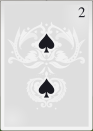
\includegraphics[width=0.75in]{images/2-of-spades.png}
	\caption{Deuce of Spades}
	\label{2spades}
\end{wrapfigure}
We are uncertain whether they consider it ``holy'' because the 22nd of the month is the usual date of the change of the sign of the Zodiac [figure~\ref{zodiac}], or if it is because the number 22 is some kabbalistic code for \textit{fellatio}, or what the baby boomers, in the Hippie days of the 1970s, would associate with the number 69, their numerological imitation of the Chinese Yin--Yang
\mbox{\begin{CJK}{UTF8}{bkai}陰陽\end{CJK}}
{\large\YinYang} [figure~\ref{yinyang}],
roughly approximating the shape of the symbol in mirror-image.\footnote{The Social Security Administration will probably have to raise the minimum retirement age to 69 in honor of these baby boomers.}  Or else there are mystical allegorical connections with drunkenness or attempts to attain, or induce or deceive or force others to attain, altered states of consciousness with mind-altering substances.

The number 22 is a double-deuce, or, as the Finns count cards (or pips on a die) \foreignlanguage{finnish}{\textit{ykk{\"o}nen, kakkonen, kolmonen, nelonen, viitonen, kuutonen,}}\footnote{Finnish: ace, deuce, trey, 4, 5, 6; all of which in Finnish are synomyms for ``devil'' as ``deuce'' is in English; as opposed to the natural counting numbers \foreignlanguage{finnish}{\textit{yksi, kaksi, kolme, nelj{\"a}, viisi, kuusi};} for which reason the Finns say that they can identify six devils, while the seventh sifts one's soul as wheat, because \foreignlanguage{finnish}{\textit{seitsem{\"a}n}} is just \foreignlanguage{finnish}{\textit{seitsem{\"a}n}}.} this would be \foreignlanguage{finnish}{\textit{kaksois-kakkonen}} rather than \foreignlanguage{finnish}{\textit{kaksi-kolmatta-kymment{\"a}}}\footnote{Finnish: literally, ``two of the third ten;'' the old way of counting, sometimes used even nowadays in ordinal form to refer to the day of the month on the calendar.} as the old ones used to count ones'-place-first up to \foreignlanguage{finnish}{\textit{yhdeks{\"a}n-viidett{\"a}-kymment{\"a},\footnote{Finnish: literally, ``nine of the fifth ten,'' or, going back to the root of the word \foreignlanguage{finnish}{\textit{yhdeks{\"a}n}}, ``one lacking of the fifth ten.''} viisi-kymment{\"a}}}\footnote{Finnish: literally, ``five-tens.''} when they shifted over to counting \foreignlanguage{finnish}{\textit{viisi-kymment{\"a}-yksi, viisi-kymment{\"a}-kaksi, jne.,}}\footnote{Finnish: literally, ``five-tens-one, five-tens-two, etc.''} tens'-place-first.  Deuce seems to be the card of lowest rank\footnote{``[C]ertain lewd fellows of the baser sort'' [Acts~17:5].} in most games, where ace is considered highest, just above king: historically, ace has been moved from the first position in numerical order \mbox{A--2--3--4--5} to the highest rank as in the straight \mbox{10--J--Q--K--A}.

\begin{wrapfigure}[10]{R}{1in}
	\centering
	
\includegraphics[width=0.75in]{images/Coat_of_arms_of_Finland.png}
	\caption{Suomen vaakuna}
	\label{eduskunta}
\end{wrapfigure}
Yin and Yang are out of balance.  Yang has been skulking about at night committing deeds of darkness outside his domain.  Yin does not rise and shine as the Sun dawning from the East when Yang has stolen her happiness in the middle of the night.  No!  Yin rises secretly, in anger, to avenge herself of Yang's violation of her body.  Yang has broken the Laws of \foreignlanguage{finnish}{Eduskunta} [figure~\ref{eduskunta}],
Judge \foreignlanguage{finnish}{Tuomari} has sentenced him to the deepest dungeon of \foreignlanguage{finnish}{H{\"a}meenlinna}, and the Great Smith \foreignlanguage{finnish}{Ilmarinen} \cite{lonnrot1849kalevala,crawford1888kalevala} is forging chains of darkness to hold him there for many Eons of Visitation.

Even here we speak of those men in suits and ties, who preach the Holy Bible one day out of seven, but twelve days out of twelve without fail, they observe in their newspapers ritualistic prognostications under the Pagan star-worship signs [figure~\ref{zodiac}].  These are the same sort of men who said John was beside himself for preaching signs in the sun, moon, and stars, the same signs already observed, mind you, by the Prophets in ancient times [Isaiah 13:10, 24:23, 60:19, Ezekiel 32:7, Joel 2:31, etc.], and for this reason almost had the Book of Revelation thrown out of the Bible at the Great Examination of the Books.

When a cabal or a powerful and secretive group of any sort begins to commit sexual assault \cite{ceasar2015}, we are not far from the most horrific cases of sexual assault ever recorded in the Bible [Judges~19:22--30], or the story of Susanna \cite{susanna}, which the scribes refused to transcribe.  It has been my experience that these kabbalists often spend a large part of the month planning, conspiring, and premeditating sexual assaults that take place with an excess frequency in the middle of the night after midnight, when the date has changed to the 22nd of the month.  Such assaults sometimes continue for the following days and nights until the assailants have satisfied their lust.

Or is it spelled ``Qabalah'' like this bizarre jewelry sales website \cite{webq}?  The men over forty \cite{over40} and the female celebrities with the red string bracelets \cite{frost2015kabbalah} simply need to take this Cabal--Kabbalah--Qabalah \textit{business}, or however else they like to spell it, \textit{elsewhere}, that is, if they don't want to end up in prison for it.  The sum total of all such business is one golden calf's worth of spiritual kitsch, compressed coal, and other such hogwash purveyed by these same whoremongers and pimps who are no doubt busy on the side trafficking in illegal drugs, murder-for-hire, and so on and so forth.  More than enough to make almost anyone vomit.

Who are these Rabbis, and where do they come from?  Even an outsider can see that they have rejected the Talmud and all the Prophets to study Kabbalah in an apparently all-consuming zeal to rid Judaism of its hated Torah and go a-whoring after graven images and strange gods and goddesses.

Who are these Rabbis, again?  Do you even have to ask?  Yes, these are the uncircumcised Realtor\textsuperscript\textregistered-preachers\footnote{In Finnish, \foreignlanguage{finnish}{\textit{lantalais-saarnaajat}}, or, in English, villein-preachers, because in truth we liken their behavior to that of the villeins of medieval Europe who would have held us in serfdom, peonage, bondage,  servitude, thralldom, and slavery all our lives long, and murdered us in cold blood if we dared pray to our Lord.} of the Old Apostolic Lutheran Church of America who preach that others must become circumcised in order to be saved.  And yes, the Law demands that they be circumcised, even that their entire members be cut off, and that they be made eunuchs, but even this will not save these preachers.  This is the same Law that demands that those unscrupulous barbers who cut or dye or perm or ``dread'' or otherwise damage, or ruin, or harm even a single human hair against the will of the human whose head it grows from, not only be scalped but decapitated as well, and that their shrunken heads be hoisted up on poles to serve as a warning and as a fitting example to others.  I will never yield one iota from this Law.

In fact we are furious about these ``Dear Brothers in the Lord'' and the alcoholic fruit soup they make of the matter.\footnote{Finnish: \foreignlanguage{finnish}{\textit{rakas velli}}, a pun on \foreignlanguage{finnish}{\textit{rakas veli}}.}
When one of these men is, err, married, to a woman, and he speaks of another man as a ``faithful laboring companion,'' we have a very uncomfortable feeling about this \cite{lollardy12}:
\begin{quote}\small
``The Third Conclusion, sorrowful to hear, is: That the law of continence annexed to priesthood, that in prejudice of women was first ordained, induces sodomy in Holy Church; but we excuse us by the Bible, for the suspect decree that says we should not name it. Reason and experience prove this conclusion. For delicious meats and drinks of men of Holy Church will have needful purgation or worse. Experience for the privy assay of such men is that they like not women. The corollary of this conclusion is that the private {\color{red}religions.\ beginners} of this sin, were most worthy to be annulled but God, for his might, of privy sin send open vengeance.''
\end{quote}
Note the typographical errors in this quote.  Unfortunately we are not able to ascertain primary sources or gain access to them.  However, we do know that when the Chinese Monkey's ninth orifice\footnote{Monkey's 9 orifices, namely: 2 eyes, 2 ears, 2 nostrils, 1 mouth, 2 lower orifices.} passes \textit{f{\ae}ces},\footnote{``O Preachers of the Fourth Period of Visitation ...''} there is no room for ``Dear Brothers in the Lord'' to enter.

No, the Lollards, famous for their ``Twelve Conclusions'' of which we have quoted the third, are not that far off from Jan Hus \cite{huss1915church}, who drew two important conclusions from the fact that a woman had actually served as pope for about two years some time during the ninth century after the birth of our Lord and Savior:  first, that a woman has the power to testify sins forgiven; and second, that neither the popes nor the cardinals of the Roman Catholic Church are infallible.  Jan Hus was burned at the stake for his conclusions.

The accepted story was that the female pope had male lovers, and in fact died in childbirth \foreignlanguage{french}{\textit{en route}} of a papal procession: that street is called ``Via Dolorosa'' in Rome in remembrance of those infamous pains of childbirth, and to this day popes superstitiously avoid it.  After the incident of the female pope, whenever a new pope was installed, he would have to sit on a special seat shaped somewhat like a modern toilet, and the cardinals would feel his private parts through the bottom of the seat and exclaim in Latin, ``\foreignlanguage{latin}{Duos habet et bene pendentes!}''\footnote{``Two he has, and well they hang!''}

The Roman Catholics deny the female pope to this day, but the words of the 15th-century French poet Franc Martin \cite{bayle1820} belie such shock and disbelief that we can scarcely doubt:
\begin{verse}\foreignlanguage{french}{
	<< O benoist Dieu! comme osa femme\\
	\noindent Vestir chasuble et chanter messe!\\
	\noindent O femme oultrageuse et infâme!\\
	\noindent Comment eust-elle la hardiesse\\
	\noindent De se faire pape et papesse?\\
	\noindent Comment endura Dieu, comment,\\
	\noindent Que femme ribaulde et prestresse\\
	\noindent Eust l'Église en gouvernement? >>
}\end{verse}

Flashing back to Franz{\'e}n's death we are reminded of that of another Swedish author, Stieg Larsson, whose satire \cite{larsson2005,larsson2006,larsson2007} of corruption within the Swedish mental health system and S{\"a}kerhetspolis (``S{\"A}PO'' \cite{sapo}, the Swedish state secret police,) earned him an early and untimely death by ``heart attack.''\footnote{The main character's breast implants in the third book of the series almost ruined it for me.  That part of the story was not fully told before the author died.  We do not believe in breast implants or shoddy medical work.}

Our work is further interrupted by clues to Edward Nelson's death.  The portrait that emerges from Princeton \cite{cook2009nelson} is an ugly one of all manner of crime and corruption up to and including bloody murder.
\begin{quotation}
... I attended first grade in Fascist Italy and still have the notebook in which I wrote to dictation, ``\foreignlanguage{italian}{Mussolini ama i bambini.}'' ... When I was twelve I took a new deck of cards and idly reordered it: ... Only the joy of making love surpasses the joy of doing mathematics, with skiing a distant third. ...

[Large photo of Nelson smoking a pipe]
\end{quotation}
The clues are everywhere.  Mafia, \foreignlanguage{italian}{La Cosa Nostra}, such an emphasis on gambling almost as if a twelve-year boy would be beaten and whipped for ``idleness'' or ``laziness'' for picking up an adult deck of cards.  Such an emphasis on love-making as to make him out to be a rapist or sex offender.  The heavy emphasis on tobacco.\footnote{Yes, smoking causes cancer, and yes, cancer kills.  We will never know whether or not smoking caused any particular case of cancer.  What we do know is that smoking heavily stacks the odds of the random mutation of cells in favor of the development of cancer.}  A biography written in the first person, but not at all clear it was written by the subject.  A total Mob scene.

We should not be surprised, given the reputation of the entire state of New Jersey as well as the neighboring New York City metropolitan area as a place where all lawful jurisdiction has been ceded to organized crime.

We do not work in the insurance industry; the closest we have come to that is to work out an alternative mathematical proof \cite{wiki2009kullbacks} of the so-called Cram{\'e}r--Rao bound \cite{cramer1946,rao1945} which has some relevance in that industry.  This was a gem \cite{fuchs1970inegalite} we had found while browsing the \textbf{NUMDAM} archives \cite{numdam}.  There are some discrepancies in those archives, because I distinctly remember the authors' phrase somewhat along the lines of, but not identical to the version of the article that I am now able to retrieve from the archive \cite[p.~119]{fuchs1970inegalite}:
\begin{quote}\small
	\foreignlanguage{french}{... l'in{\'e}galite de Cramer--Rao r{\'e}sulte imm{\'e}diatement de celle de Kullback.}
\end{quote}
But the proof immediately following in the current version of that article was missing from the version of the article I retrieved some years ago from \textbf{NUMDAM}, and now shivers run up and down my spine because an acute accent or two is missing, most conspicuously from Cram{\'e}r's name.  Nor is that phrase on the same position on the page that I remember.

From an insurance perspective, when the rate of mortality in some particular geographical area, cohort, or field of study or work is greater than what would be considered a natural mortality rate, and the excess deaths lack a satisfactorily attributable cause, then an insurance investigation is called for, particularly when the excess deaths would in any event affect premiums for life, health, and accident coverage, and, if the true cause of the excess mortality is not determined and redressed, place the solvency of insurance companies offering such coverage at stake.

Those who do work in the insurance industry are generally not at liberty to speak of such matters.

\subsection{The Lunatic}\label{lunatic}
When I was a small child, I asked my grandfather, ``What is a cult?''

``Why do you want to know?'' he asked me.

``They told me at school that our church was a cult,'' I replied.

My grandfather sighed, and told me about the \foreignlanguage{finnish}{\textit{Urantia-kirja}}\footnote{The Urantia Book was so unearthly strange that, except for issuing a formal command not to read the book, ``\foreignlanguage{finnish}{{\"A}lk{\"a}{\"a} lukeko t{\"a}t{\"a} kirjaa pyh{\"a}ksi raamatuksi!}'' the Old Ones were so uncomfortable speaking about it in their own tongue, that they used other language to describe the book, and they called its Fifth Epochal Revelation a ``period of visitation.''  Then they denied its existence, mocked the Urantia preachers for their inability to count, and told them there were only four periods of visitation. To this day the fourth and final period of visitation is preached in defiance of Urantia.} \cite{urantia-kirja}.  ``Don't ever join a cult,'' he said.

Not so long ago, in my church, a new book was published in English.  All we find of it online is an obscure and misspelled citation \cite{hagglund1994religious} to an edition that came out in the Finnish language in the 1960s:
\begin{verse}
``LAESTADIUS, L.\ L.\ (1968), \foreignlanguage{finnish}{\textit{Hulluinhuonelainen}} \foreignlanguage{swedish}{(D{\"a}rhushjonet)} (The Bedlamite [Finnish translation]) trans.\ \foreignlanguage{finnish}{L.\ Mustakalio, Joensuu,} Finland: \foreignlanguage{finnish}{Akateemian Kustannusliike.}''
\end{verse}
There are several discrepancies. The title of the Swedish edition correctly ought to be spelled \textit{D{\aa}rhusjonet}.  The English edition (which came out much later) is called \textit{The Lunatic}, rather than ``\textit{The Bedlamite},'' unless there is an older English edition of which I am unaware, which seems entirely possible to me.   The publisher cited is either unknown or a misspelling or alternate spelling of ``Akateeminen\footnote{Finnish: \foreignlanguage{finnish}{\textit{akateeminen}}, academic or scholarly, etc.; an adjective in the nominative case: more neutral in connotation than \foreignlanguage{finnish}{\textit{akateemian}}, genitive (possessive) of the noun \foreignlanguage{finnish}{\textit{akateemia}}, if not a ``true cognate'' to academy, at least a school or college or some other alleged institution of training, instruction, or education; hence ``Academy's Publishing Concern, Inc.'' implying some association with an academic institution that probably does not even exist.} Kustannusliike\footnote{Finnish: \foreignlanguage{finnish}{\textit{kustannusliike}}, publishing concern.} Oy\footnote{Finnish: \textit{Oy}, standard abbreviation for \textit{\foreignlanguage{finnish}{Osalliyhdistys}}, a share corporation, ``Inc.''}'' \cite{google2016akateeminen}, which is somewhat ironic, because I see little or nothing academic about this publisher.  A standard \texttt{whois} query of the domain associated with that business reveals little more that the Google search \cite{google2016akateeminen} except for an apartment or suite number A~5 at the same street address, and two very common family names, Tapani and Mattila, almost as if the Smiths would have christened their child Jones after the neighbors...  No, I don't think so.  I call baloney\footnote{Swedish \textit{falukorv}, not to be confused with Italian \textit{bologna}.} on that.  It could even be some random cohabiting couple like a million others in that city, who have never even heard of \foreignlanguage{finnish}{\textit{Hulluinhuonelainen}}.

The Finns have ``movements;'' hence the Finnish word \textit{liike}, a ``movement,'' that is, a political or emotional or spiritual movement.  These publishers might have made a public announcement something like, ``There has been a movement to publish a new edition of such-and-such a book.''  In this case a ``movement'' would be more like what the business class would call a ``single-purpose entity'' \cite{rixon2015spe}.  I would venture so far as to guess that the URL \url{http://spes.fi/} \cite{google2016akateeminen} overtly refers to the acronym ``SPE'' for the phrase in English.

One cannot even say something like, ``Let's go!'' literally in Finnish: that would be \textit{L{\"a}htek{\"a}{\"a}mme!} (``Let us depart!'') language so formal you would never use it unless you were Moses stretching forth your staff over the Red Sea.  No, the Finns use the passive voice of an unspecified human agent, in the present tense of the indicative mood, to express such a command,  \textit{L{\"a}htet{\"a}{\"a}n!} (``People are leaving!'') in an almost mobbish ``suggestion'' that ``we'' had better be leaving, too, along with these unspecified humans.\footnote{Finns are stubborn.  One does not just ``tell'' them what to do.}

\textit{The Lunatic} begins with a strange railing argument that physicians have more insight into the human soul than philosophers do.  I cannot hold \textit{The Lunatic}, a.k.a.\ \textit{The Bedlamite}, as a true work, and consequently I cannot remain in good conscience in the church that publishes this book and insists it is a true work, or for that matter the state that publishes volume after volume of such lunacy \cite[etc.]{rcw-10.77,rcw-71,rcw-72.06,rcw-72.23,rcw-72.27,rcw-72.25,rcw-72.29,rcw-37.12.010.4,bigfoot1969,bigfoot1984} and enforces it as law with gunfire, imprisonment, lethal and non-lethal injection, and all manner of hideous torture, in some grotesquely perverted pretense of ``justice'' and ``healing.''

\textit{The Lunatic} is intended for those who consider themselves intellectuals within the church to read.  Its theme is an occult mixture of psychology, psychiatry, and religion so strange that it verges on witchcraft, with some leanings toward agnosticism or even atheism.  There is a certain line of thinking in this book, at odds with mainstream Christian doctrine, that the soul is seated in the brain \textit{and therefore ceases to exist at brain death}.  Our objection to this is that if this is what people believe, there is nothing to prevent them from saying so openly as many others freely do without the occultism.  But at the same time they want others to think of them as Christians, when they themselves no longer believe in heaven or hell.

Furthermore the book is used to justify serious human rights violations within the church via an occult practice of psychiatry and psychology mixed with religion, which has become \textit{de rigeur} today, especially within Catholicism \cite[etc.]{catholicpsych,kugelmann2011}.  We are essentially reporting that this same disease has spread to Lutheranism.  We demand in all cases that federal and state government cease funding and enforcing religious conversion therapy that takes place under the cloak of the practice of psychiatry and psychology, and that those who practice such therapy be disgraced from religious ministry.

Another theme running through \textit{The Lunatic}, which we find alarming, is that of excessive and forced intimacy between parents and children, to the point of molestation and abuse of minor children, leading to medieval-level villeinage and bondage of adult children, brutally enforced obedience to Mafia godfathers, etc.

There is a higher law, even as the elders have said, ``God's Law breaks all other laws.'' While I believe in one God Who can and will eternally punish those who break His Law, I do not demand that others believe in Him: I believe that even those who do not believe in God, or do not know that God exists, will see even an atheist or agnostic sense of justice fulfilled in the punishment of those quacks, shrinks, and shysters already in this life for violating the Laws of Nature and the unalienable rights of their fellow human beings, and they will know that God is there.  So may the remainder of the natural lives of these disreputable physicians, psychiatrists, and lawyers be a foretaste of the eternal damnation they face, just like the earthly punishment they have decreed for their innocent victims, whose unearthly screams have ascended from the mental hospitals all the way to heaven, even to the ears of the Lord of Sabaoth, who is coming in great wrath, indignation, and fury to visit the vengeance of His mighty armies upon those quacks, shrinks, and shysters, and all others who hold to their side for the blood of His innocent children whose tortured screams He has heard.

As to the argument in \textit{The Lunatic},\footnote{How do we respond to this argument when the book is suppressed, all but banned, as it were?  Do the Jews suppress the \textit{Protocols of Zion}?  No, where is the book, that all may read, and all may judge?} in the first place, philosophers are much better than physicians at doing no harm, and in the second place, physicians need to have their thinking cap on straight before they start doctoring others' bodies or worse, their minds.  I have never been injured, sickened, or hurt by a philosopher's contemplations.  Nor has anyone else.  If I think they are idle or useless, or if I don't want to listen to them or read them, I don't have to.  No philosopher is forcing me.  

Physicians on the other hand are traditionally under oath \cite{north2002hippocratic}, I quote, to
\begin{quote}
``... do no harm or injustice ...''' 
\end{quote}
to their patients.  Yet the first thing a physician does whenever he or she sees a new patient, even a newborn child, or a patient of any age, male or female, is to make some plan to cause permanent and lasting harm to that human being; the physician then carries out this plan with deliberation and malice.  Unnecessary dental work, unnecessary surgeries, and toxic and unnecessary drugs characterize medical practice today; and those treatments which are necessary and beneficial are totally denied to the masses, to whom this is all that they offer:
\begin{itemize}
\itemsep0em
\item Circumcisions: all but mandatory for all baby boys, whether they are Jewish or Muslim or not;
\item Botched and unsanitary immunizations;
\item Dental exams, fillings, root canals, crowns, tooth extractions, bridges, dentures, \$\$\$;
\item Access to ``controlled substances;'' and
\item Civil commitments of political dissidents and wayward family members.
\end{itemize}
Physicians as they practice today are first and foremost thieves, and as Jesus said, ``The thief cometh not, but for to steal, and to kill, and to destroy'' [John 10:10].  If they don't steal, they rob; if they don't rob, they murder; if they don't murder, they drug; and if they don't drug, they torture.  Their wrongdoing goes far beyond even the most vicious, grisly, and aggravated murders we ever read about in the newspapers.  When war crimes tribunals are held over these doctors, the jurors who hear the evidence of their crimes will have nightmares for the rest of their lives, and they will surely be hanged.  In the meantime we have to be satisfied with a slap on the wrist for these war criminals \cite{osullivan2016western}, but those that have passed and continue to maintain such vicious laws  \cite[etc.]{rcw-10.77,rcw-71,rcw-72.06,rcw-72.23,rcw-72.27,rcw-72.25,rcw-72.29,rcw-37.12.010.4,bigfoot1969,bigfoot1984} in the first place have yet to be punished for their treason:  being the drug dealers they are, they refuse to take no for an answer, when a patient would dare refuse such a harmful and unsalutary regimen and demand respect for those unalienable rights enumerated in the founding documents  \cite{found} by our forefathers. Those traitors have deeply corrupted society with sick, twisted, and corrupt laws, worthy of Holocaust-era Germany, so that they can ``legally'' hold their victims \foreignlanguage{spanish}{incommunicado},\footnote{Spanish:  \foreignlanguage{spanish}{\textit{incommunicado}}, unable or not allowed to speak or communicate with others or forcibly prevented from doing so.} in physical and chemical restraints, and forced to endure even more drugs and horrific torture.

As if that were not enough, they deprive their victims of their civil rights \cite{rcw-9.41.040} for the rest of their lives even after forcing them to endure such horrific torture; even if state law were to provide an effective process for restoration of rights \cite{wac-388-865-0585}, this possibility is all but entirely foreclosed by \textit{federal law} which denies these rights \textit{for life} to any person who
\begin{quote}
``...  \cite[\P\P(d)(4),~(g)(4)]{18usc922} has been adjudicated as a mental defective or has been committed to any mental institution;''
\end{quote}
affecting far out of any just or reasonable proportion those who are of LGBT, Jewish, Black or other minorities.  So much for the doctors' promise to do no injustice; and that part goes for \textit{Juris Doctor} as well as \textit{Medicin{\ae} Doctor}.  From a computer programming perspective this U.S. Code exhibits \textit{at least four} classic \textbf{smells} \cite{fowler2006codesmell}: duplicate fragments \cite{sourcemakingdup}, bloat \cite{sourcemakingbloat}, change preventers \cite{sourcemakingchangepreventers}, and excessive coupling \cite{sourcemakingcouplers}, namely between federal and state code.  This \textbf{odor} has reached the level of a general \textbf{stench} in Washington, D.C.

Do you recognize that code smell?  The Germans sure do.  It is the smell of burning human flesh mingled with the miasma of rotting corpses that rises from the foul waters of the Potomac River.  Those who force us to wear the black triangles of the aforementioned Title 18 U.S.C., \S922, \P\P(d)(4), (g)(4), along with the falsified and embellished public records of civil commitment proceedings which were held not in open court but in secret torture chambers, are war criminals: let them be so charged.

After the black triangles come the pink triangles and yellow six-pointed stars, if history be any guide.  Next they will ship us humans on cattle cars to concentration camps.  Let us call an immediate halt to this business, and set it right as soon as possible to mitigate the massive loss of human life which inevitably follows such unredressed evil.

And as war criminals do, they deny, excuse, apologize, and minimize.  They want to deny me my rights for purported reasons of \textit{public safety}?  What a vicious slur against my character!  What libel, what slander!  As if I'd be a murderer if I had ``access'' to a weapon or a job or a home!  What other excuses do they have, now?  I am driven far from my previous home and from town to town by mobs with gunfire, denied access to public libraries and federal government offices, falsely arrested, beaten, robbed, and pick-pocketed, time and time again.  Yet the permanent disability imposed by Title 18 U.S.C., \S922, \P\P(d)(4), (g)(4), remains without redress.

Let those war criminals answer for themselves.  I want them to pay damages, fines, compensation, restitution, and reparations for the wrong they have done and will continue to do as long as they are not punished for it.  I want them to lose their freedom because they held mine so cheap.  I want all my rights, every last one of them, recognized and fully restored.  As a citizen of the United States, this is my birthright \cite{found}, and this is what I demand.

I have preached hell and condemnation.  Do not ask me about heaven.  You held my soul cheap and practiced \textit{psychiatric conversion therapy} on it.  You may ask Jesus, ``Lord, when saw we thee an hungred, or athirst, or a stranger, or naked, or sick, or in prison, and did not minister unto thee?''  Do not ask me to ``accept'' what I ``cannot'' change.  Your ``can't'' and your ``won't'' are alike an abomination to me.

You Realtor\textsuperscript\textregistered-preachers don't even ask forgiveness for your sins any more.  You have amassed so much real estate by crooked dealing that you beg the Heavenly Father, ``Forgive us our trespasses,'' when you feel some twinge of regret that you might have stepped on the your neighbor's property by mistake while you were setting a fence post.  No different, really, from the young man who suddenly feels guilty for listening to the radio in the car because he has picked up a prostitute.

There isn't enough room in Battle Ground for your cattle, so just like the \foreignlanguage{finnish}{\textit{lantalaiset}}\footnote{Finnish: \foreignlanguage{finnish}{\textit{lantalainen}}, land-owner, villein, or settler.} of old you drive out even your own kin as if they were \foreignlanguage{finnish}{\textit{lappalaiset}}\footnote{Finnish: \foreignlanguage{finnish}{\textit{lappalainen}}, Lapp or Sami.} or \foreignlanguage{finnish}{\textit{mustalaiset}}\footnote{Finnish: \foreignlanguage{finnish}{\textit{mustalainen}}, Gypsy or Romanian; a racial slur.} to make more room for yourselves.

Jesus preached the Gospel to the poor.  You preach Realty\textsuperscript\textregistered\footnote{To the best of my knowledge the words Realtor\textsuperscript\textregistered\ and Realty\textsuperscript\textregistered\ are actually registered as trademarks --- believe it or not --- by two \textit{different} companies, a for-profit and a non-profit, whose relationship is somewhat like that of the couple next door who talked to some therapist or counselor shrink out of Paris, France and found out they are in ``compulsion'' with each other, and now they are looking for a third party to compliment them for not suing each other for divorce, and oh, by the way, please don't report them to Child Protective Services for exposing their children to all the orgies with those strange people who keep visiting.  In other words, their legal position is not very strong in these registered trademarks.}  to the masses, complete with short plats \cite{rcw-58.17.060}, title insurance, mortgages, conditions, covenants, and restrictions.  And yet you have the nerve to mock the pre-Christian Sami for worshipping a certain stump in the ground in Swedish Lapland.\footnote{They had various rituals, and one possible explanation is that in those days it may have been a matter of life or death to orient oneself to the location of a certain stump or other landmark, and be able to find one's way back at a later time or date to that same location on the tundra.}  You are no different from the Mormons who preached the holy Plat of Zion \cite{williams2016revised} in the plains of Utah. Is this the voice of one crying in the wilderness \cite{laestadius1988voice}?

And for all that, none of you recognize the reference to some obscure passage of Scripture [Isaiah~40:3] that you have never even heard of before, because it is not in the canon of ``familiar places'' of Scripture that you are allowed to speak on.

Daughters of Sodom always flock to such Realtor\textsuperscript\textregistered-preachers.  I have no sympathy for you, either, when you refuse to strengthen the hand of the poor and needy and commit abomination before the Lord [Ezekiel~16:49--50].  What do you gain by your plain appearance while your brethren are patronizing prostitutes?  You may as well put on the jewelry of Qabalah \cite{webq}, let the females at the Ulta beauty salon teach you how to apply make-up, and let other females ``do'' your hair, and fingernails, and still other females give you pedicures, the sort who will sneak into your bed at night and clip your toenails while you are asleep if you don't watch out for them.  Oh, do you need medical care?  Just visit the female OB/GYN at the Women's Health and Beauty Spa\footnote{I suppose they perform routine hysterectomies there, not unlike the routine FGM or ``female circumcision'' which to this day is practiced by witch doctors \foreignlanguage{french}{\textit{{\`a l'Afrique}}}.  Oh, yes, these doctors practice in the United States.  They cut off the \textit{clitorides} of 12-year-old girls, and most of them are men with M.D. or D.O. degrees who pant like dogs all the while they are performing this vile operation.  Not unlike those mental health therapists who say to their resident psychiatrist, ``I have a client with boner disease, and I need a Doctor of Osteopathy to fix that.''} in San Francisco\footnote{Cities such as San Francisco, California and Toronto, Ontario are known for their promiscuous homosexual activity, which takes place in public bathhouses or saunas.} or Palm Desert,\footnote{A resort town.} California.  Your Realtor\textsuperscript\textregistered-preachers are the same ones who preach homosexuality to be a sin.  Just ask them what to do.  You people all brought this on yourselves.  Can't you make it right yourselves?  Are you jealous?  Do you want to look like those hookers or prostitute yourselves?

Not so many years ago, the people in that area would visit \foreignlanguage{spanish}{Los Algodones} for health care, because it was safer and cheaper in that town, but they would be careful to check the backgrounds of the doctors.  But \foreignlanguage{spanish}{Los Algodones} is in \foreignlanguage{spanish}{Baja California}, Mexico and these days it is getting dangerous to cross international borders, and recently I have heard rumors of unscrupulous doctors showing up in that town with connections to criminal cartels.

Men's health care?  Do men need health care?  Oh, just buy those male enhancement pills they sell at the gas station, unless you have AIDS or cancer or something like that.  They do offer free STD tests at the men's clinic in that part of town.

You see, when you preach Realty\textsuperscript\textregistered, you \textit{force} homosexuality, prostitution, abortion, and many other similar and related things upon the Christians.  What can I say about these things?  You may as well read the 137th Psalm to its bitter end.

On the male side, you preachers are running a San Francisco barbershop, and you sing a Chinese quartet,\footnote{The Chinese are superstitious of the number four.} like the intersection, as close as I can tell \cite{googlemaps2016battle}, of NW 10th Avenue, a.k.a.\ NE 122nd Avenue, a.k.a.\ NE Lewisville Highway, a.k.a.\ State Route 503, with NW 25th Street, a.k.a.\ NE 244th Street, in Battle Ground, Washington, where your churchgoers had installed a traffic light, and there was a complaint of a serious accident with injuries because the traffic light was green all four ways.

And how did you advise those construction contractors, when they had received a letter from the Army Corps of Engineers, ordering them, by authority of the Department of the Army, to halt work on some construction project or another?  In many cases the rest of us were left to wonder what really happened and how and why that work continued in spite of the order.

Now that we are speaking the language of California, you cannot give the gangsters\footnote{The word \textit{gang} is reminiscent of the Chinese expression \textit{gung ho}, ``people working together.''  In any case, gang-related crime is organized crime.} of Los Angeles\footnote{Los Angeles, California is known for its criminal gangs.} a San Francisco haircut, and then expect the rest of the world to accept them as perfect little angels because they are so clean-cut.  Yet this is what you do, and this is your religion and your church in Battle Ground.  And now you want to have \textit{korkea messu} after you have taken all the Finnish songs out of the songbook \cite{hymns}.

I want no part of it, and I don't care what your politics are, either, whether you are Dixie Democrats or greedy rich Republicans.  You preachers tell your parishioners that they will go to hell if they go to the ``heresy'' church, and their preachers tell them they will go to hell if they go to your church.  Meanwhile we find out that the preachers of both churches are meeting together like the Grand Dragons of the Ku Klux Klan in some lodge with white hoodies plotting to burn wooden crosses this Christmas.  I'll tell you what.  You can all go to hell together.  Leave me out of it.  You have made it your religion to wickedly torture and heavily burden us, the innocent ones,\footnote{We speak of the innocent ones; others speak of indigo children, targeted individuals, etc.} for the entire duration of our existence on this earth.  So let it be done to you for eternity.

And as to the aforementioned Title 18 U.S.C., \S922, \P\P(d)(4), there is no dawn's early light as long as an evil statute like this stands on the books.  You who passed this law have forever extinguished the lights of liberty, and replaced our beloved national anthem with the 137th Psalm.  As you have done to us, the innocent ones, so let it be done to you for eternity.  The flag of the United States of America will never be raised by my hand or on my property, nor will my voice ever be heard to sing the \textit{The Star-Spangled Banner} \cite{key1814star}, as long as a wicked law like that stands on the books, and as long as those who passed it and continue to maintain it and enforce it have not rendered due account for their evil deeds.
\begin{figure}
\noindent\begin{minipage}{0.45\textwidth}\centering
	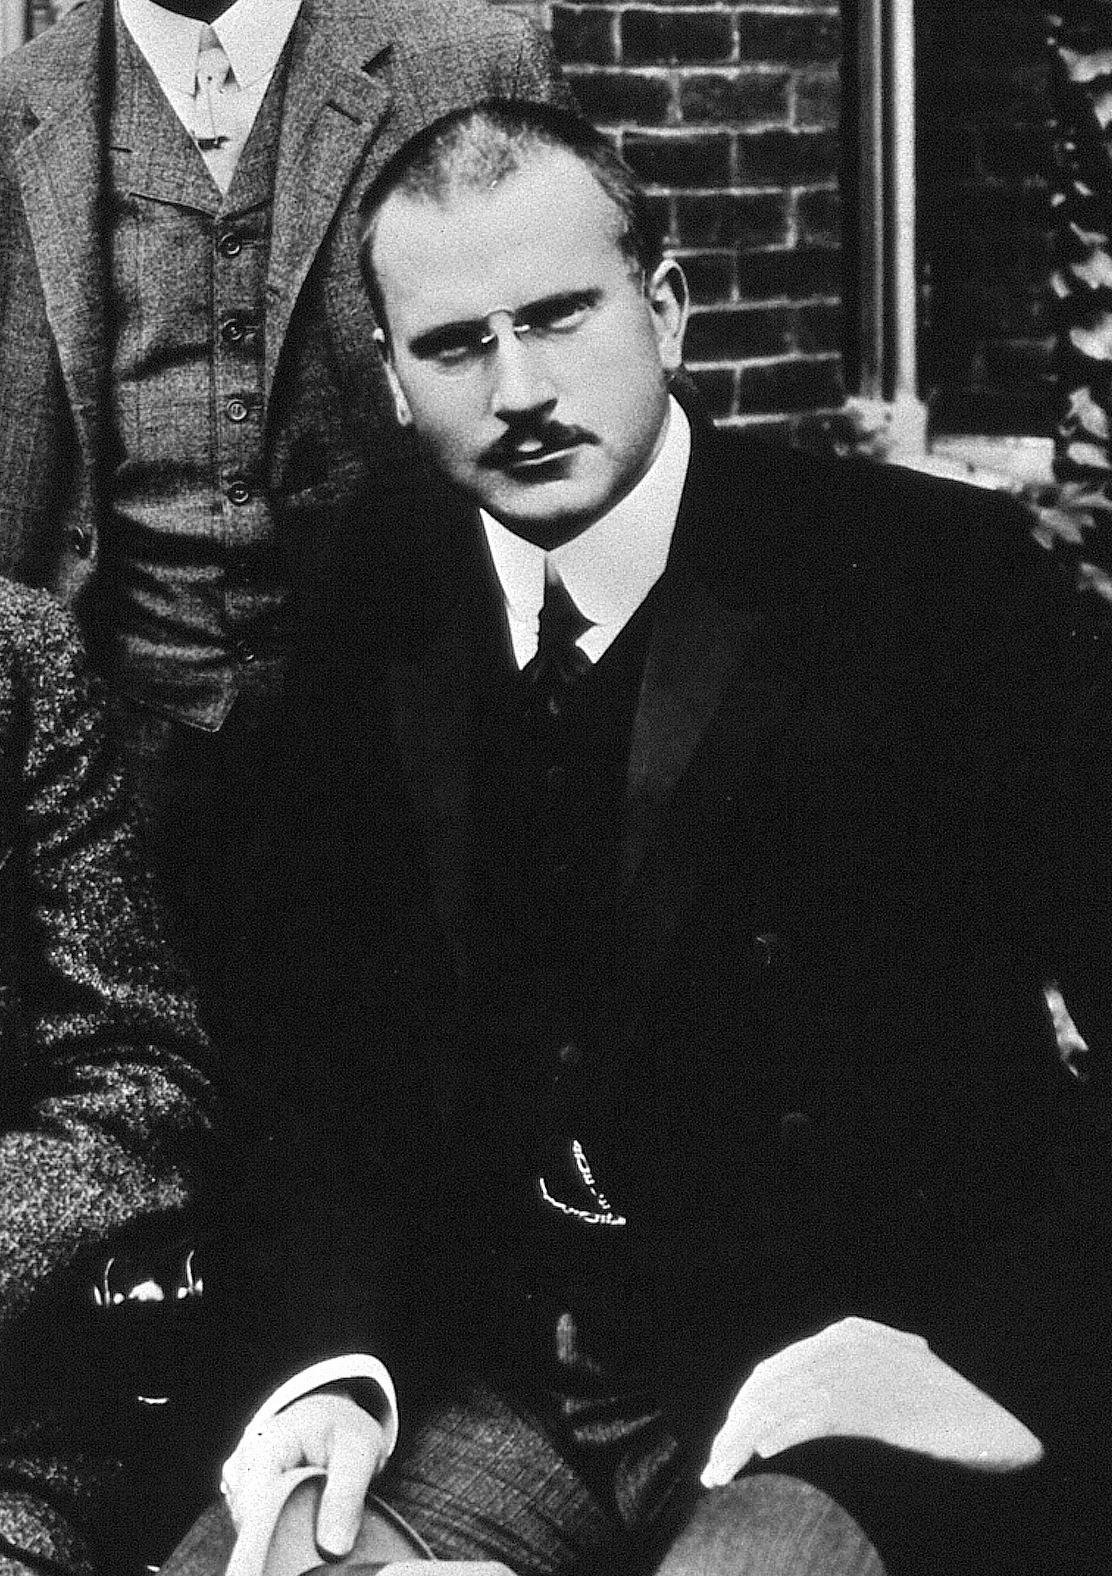
\includegraphics[width=1.0\textwidth]{images/Carl-Jung-mod.jpg}
	\end{minipage}\hskip 0.10\textwidth\begin{minipage}{0.45\textwidth}\centering
	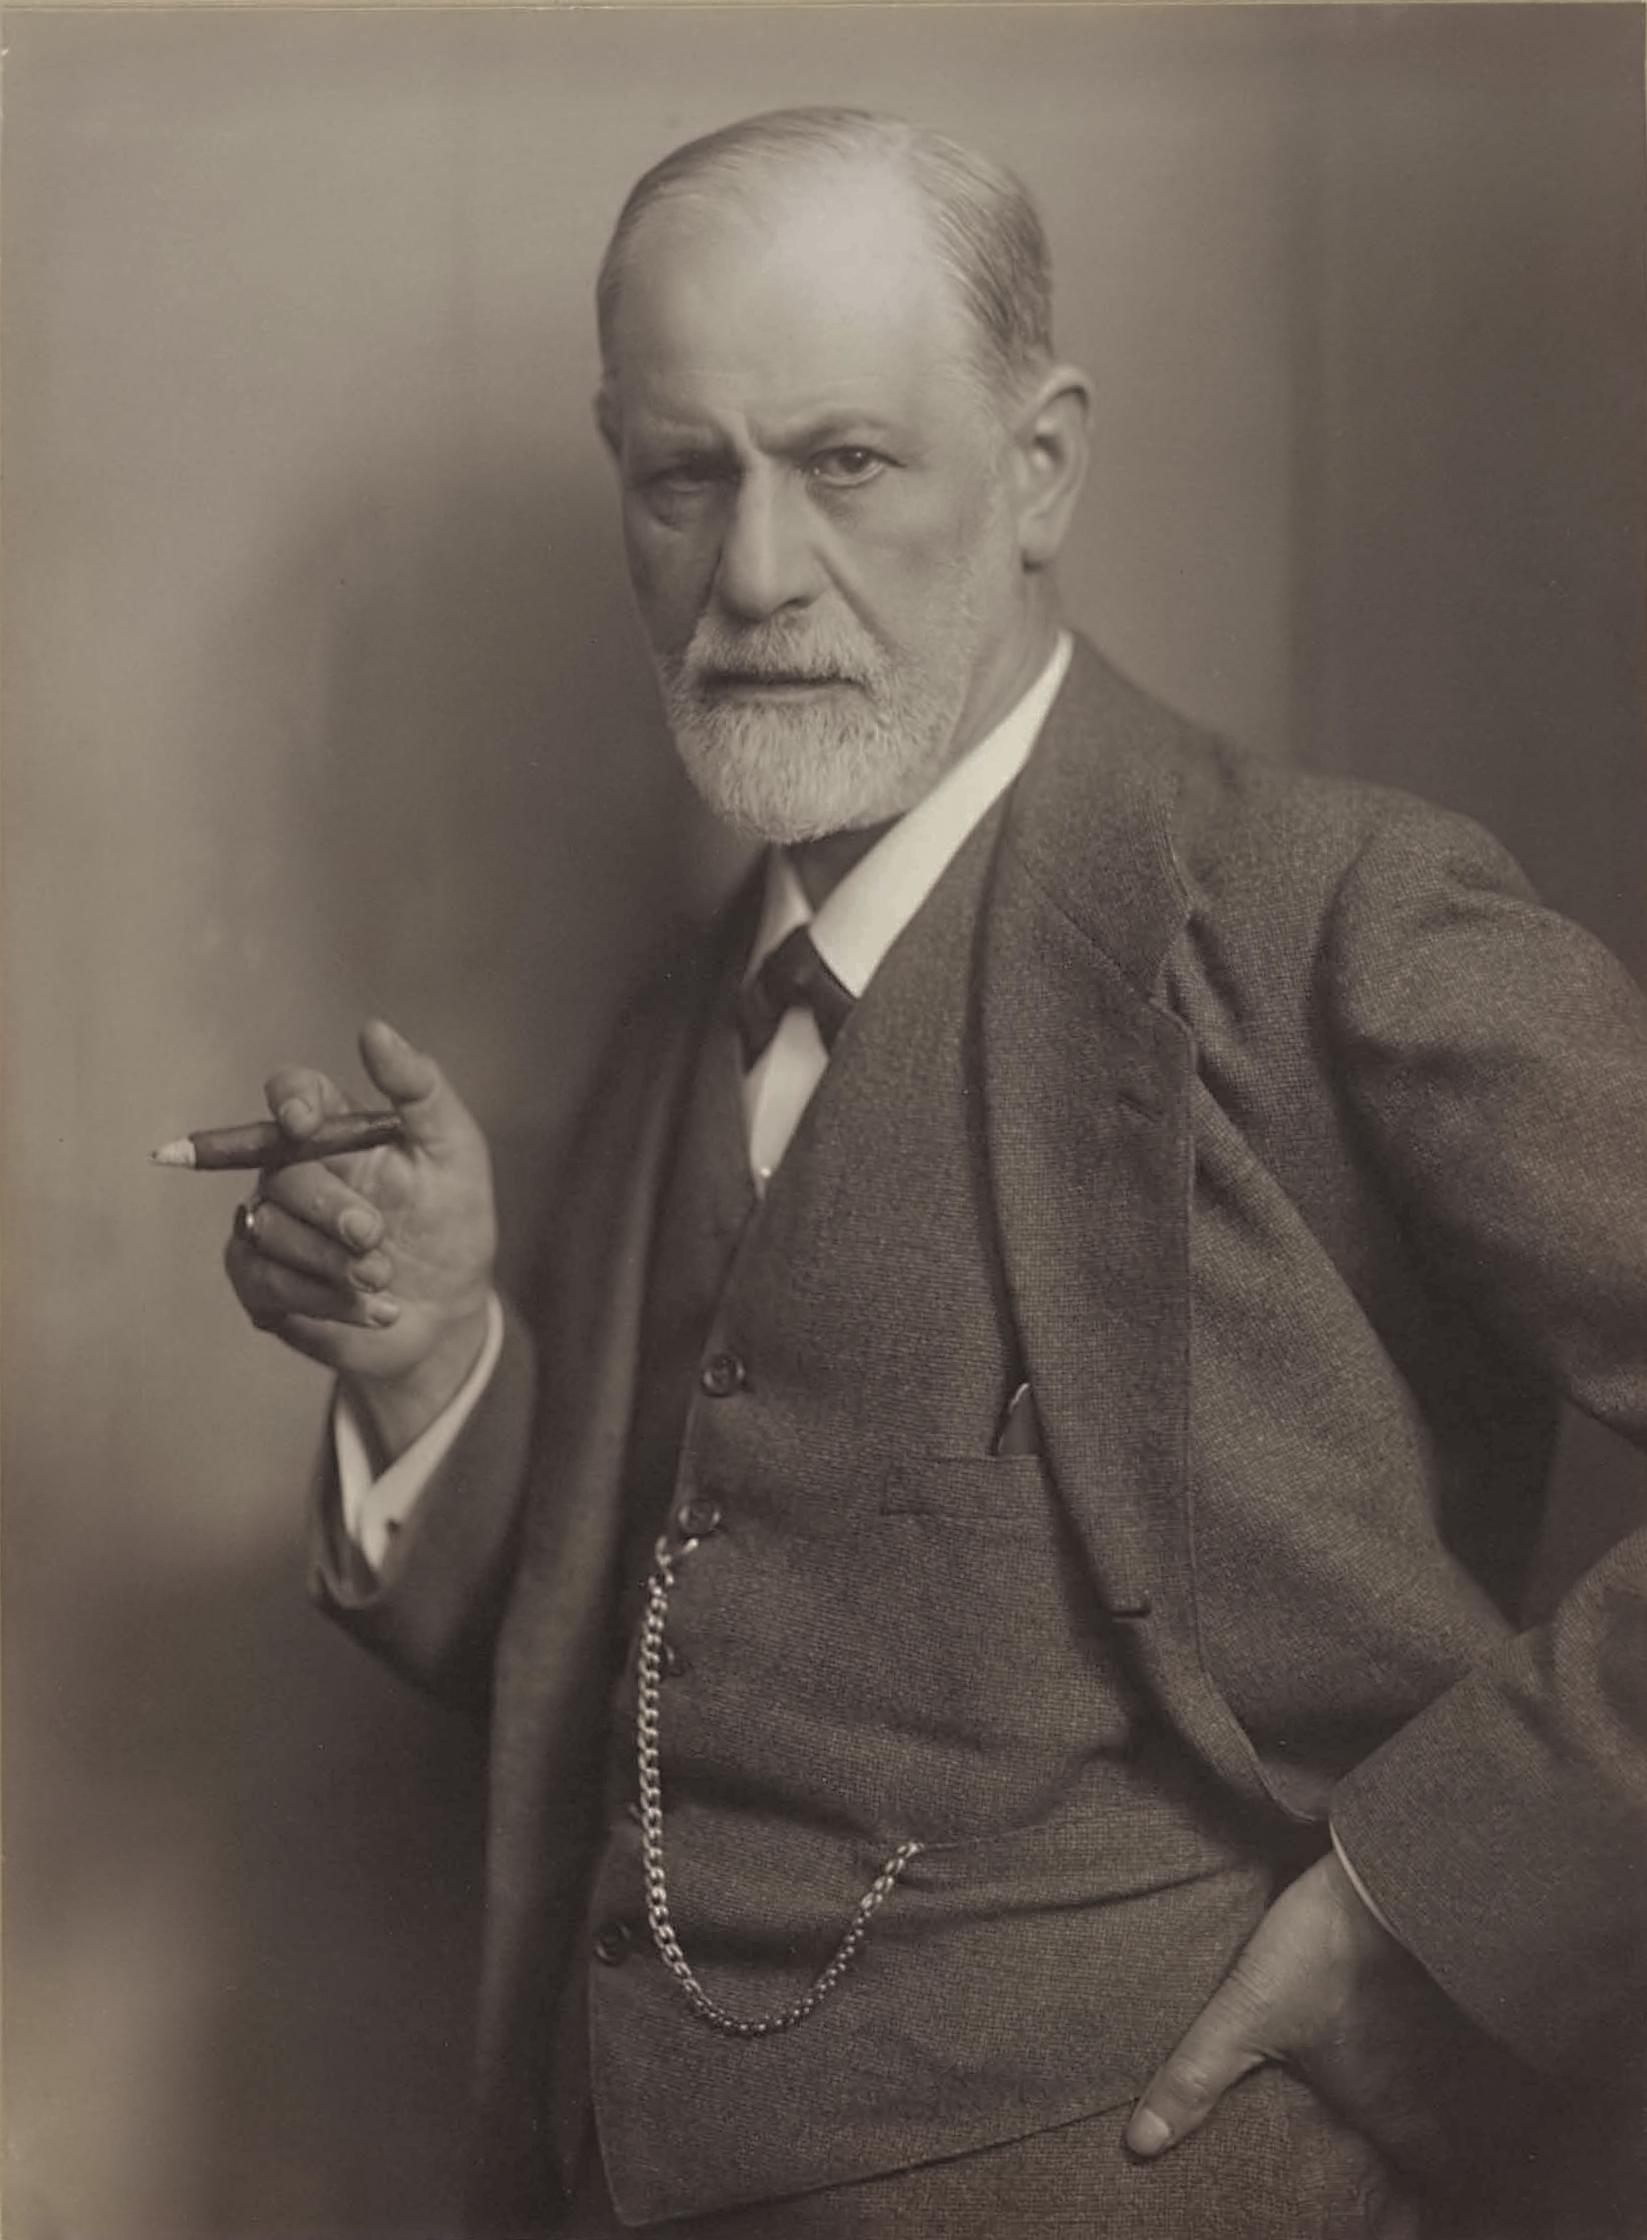
\includegraphics[width=1.0\textwidth]{images/Sigmund_Freud.jpg}
	\end{minipage}\\
	\noindent\begin{minipage}{0.45\textwidth}\centering
	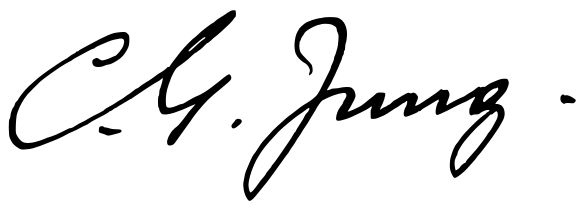
\includegraphics[width=1.0\textwidth]{images/585px-Carl_Jung_signature.png}
	\end{minipage}\hskip 0.10\textwidth\begin{minipage}{0.45\textwidth}\centering
	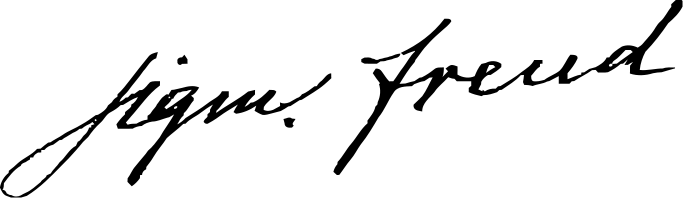
\includegraphics[width=1.0\textwidth]{images/683px-FreudSignature.png}
	\end{minipage}
	\caption[Adjudicated as a mental defective]{Pre-WWI Austrian psychiatry \cite{unknown1909,halberstadt1940,jung-sig,freud-sig,jung-sig-src,freud-sig-src}: ``Adjudicated as a mental defective.'' Unlawful to possess a firearm or any ``ammunition'' \textit{for life} under penalty of fines and up to ten years' imprisonment.}
\end{figure}

\begin{figure}
\noindent\begin{minipage}{0.45\textwidth}\centering
	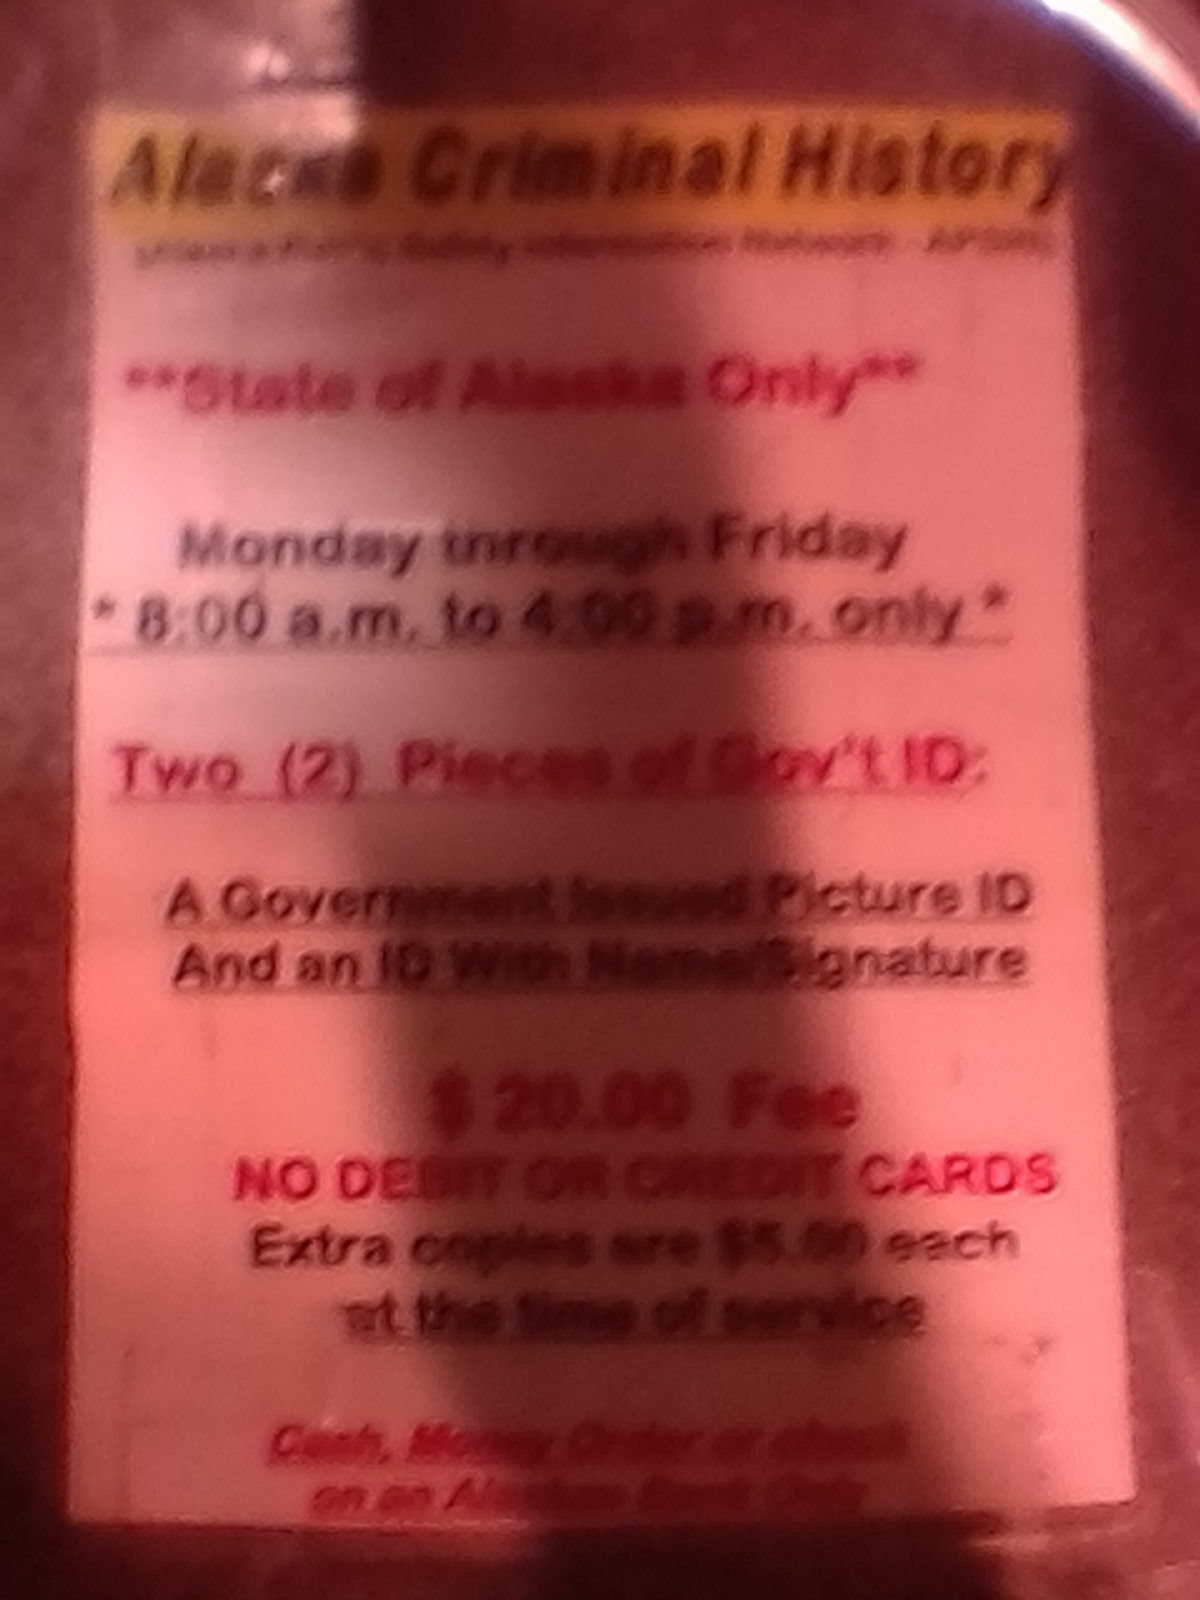
\includegraphics[width=1.0\textwidth]{images/IMG_20171206_151214.jpg}
	\end{minipage}\hskip 0.10\textwidth\begin{minipage}{0.45\textwidth}\centering
	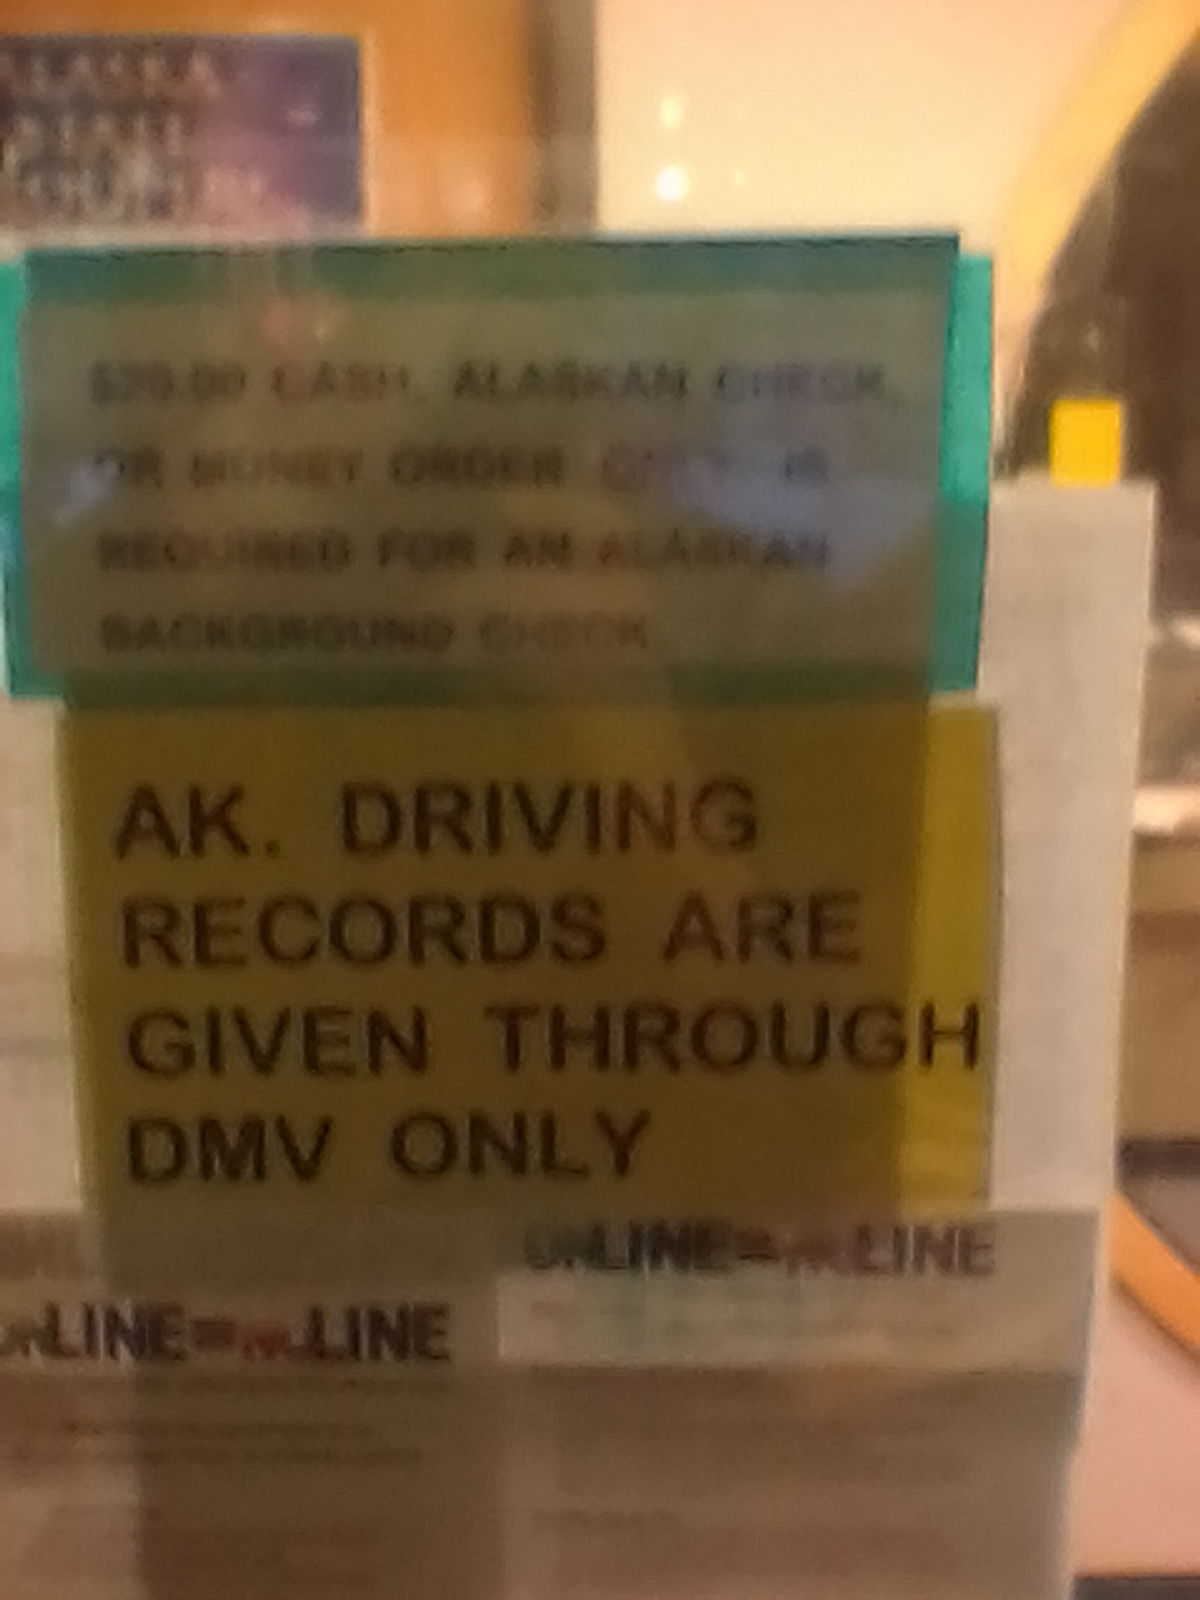
\includegraphics[width=1.0\textwidth]{images/IMG_20171206_151246.jpg}
	\end{minipage}
	\caption[Fee-for-service records]{Fee-for-service record \cite{asp2017}: ``Oh, no, we didn't include \textit{those} records.  That's another \$20 from another department, and if we ever catch you with a firearm you will be imprisoned for life if you aren't shot on sight!''}
\end{figure}
\subsection{Modern Internet companies}
I do not ``fit in'' with this exclusively male crowd. 

Oracle \cite{orcl2016} attracts a certain worshipful following who spend a lot of their clients' money on it while scorning free and open source alternatives such as MariaDB \cite{mariadb2016} and Postgresql \cite{postgresql2016}.

Google \cite{page2016alphabet} has recently reincorporated under the name ``Alphabet, Inc.,'' stripping its iconic GOOG stock of voting rights, which were split off into shares of a different class trading under the symbol GOOGL, wherein the founders have further consolidated their control of the company.  Furthermore, the very name ``Google'' is reminiscent of men's eyes bugging out while they pant like dogs looking up all the smut indexed by the great search engine.

Amazon \cite{amazon2016} is named after some mythical tribe of female warriors in South America, who supposedly cut off their right breast so it would not get in the way when they drew a bow with their right hand to shoot an arrow.  The word can be broken down to ``a-,'' a Greek privative, and ``-mazon,'' related to the root ``mast-'' as in ``mastectomy.''

Facebook \cite{facebook2016}:  I refuse to read a book with my cheeks buried in the pages.  I prefer a minimum $14''$ comfortable reading distance.\footnote{On this note I have enlarged the font of this working copy to make for slightly more comfortable reading.} Face. Book. Vomit.  I am simply sick of all the bullshit, and unfortunately cow excrement does not smell any better than bullshit.

\phantomsection\addcontentsline{toc}{section}{References}
 \bibliography{pnp}{}
\end{document}
